% This must be in the first 5 lines to tell arXiv to use pdfLaTeX, which is strongly recommended.
\pdfoutput=1
% In particular, the hyperref package requires pdfLaTeX in order to break URLs across lines.

\documentclass[11pt]{article}

% Change "review" to "final" to generate the final (sometimes called camera-ready) version.
% Change to "preprint" to generate a non-anonymous version with page numbers.
\usepackage{acl}
\usepackage{lipsum}
% Standard package includes
\usepackage{wrapfig}
\usepackage{times}
\usepackage{latexsym}
\usepackage{enumitem}
\usepackage{enumerate}
\usepackage{graphicx}
\usepackage{subcaption}
% For proper rendering and hyphenation of words containing Latin characters (including in bib files)
\usepackage[T1]{fontenc}
% For Vietnamese characters
% \usepackage[T5]{fontenc}
% See https://www.latex-project.org/help/documentation/encguide.pdf for other character sets

% This assumes your files are encoded as UTF8
\usepackage[utf8]{inputenc}

% This is not strictly necessary, and may be commented out,
% but it will improve the layout of the manuscript,
% and will typically save some space.
\usepackage{microtype}

% This is also not strictly necessary, and may be commented out.
% However, it will improve the aesthetics of text in
% the typewriter font.
\usepackage{inconsolata}

%Including images in your LaTeX document requires adding
%additional package(s)
\usepackage{graphicx}
\usepackage{booktabs}
\usepackage{longtable}
\usepackage{float}
\usepackage[utf8]{inputenc}
\usepackage{pifont} % for shape symbols

% Define short commands for each shape
% \newcommand{\affcircle}{\ding{108}}  % ●
% \newcommand{\affsquare}{\ding{110}}  % ■
% \newcommand{\affdiamond}{\ding{117}} % ◆
% \newcommand{\affstar}{

% If the title and author information does not fit in the area allocated, uncomment the following
%
%\setlength\titlebox{<dim>}
%
% and set <dim> to something 5cm or larger.


% \newcommand{\vt}[1]{{\color{blue} [VT: #1]}}
% \newcommand{\fb}[1]{{\color{magenta} [FB: #1]}}
% \newcommand{\lh}[1]{{\color{cyan} [LH: #1]}}

%\newcommand{\tbd}[1]{{\color{red} [#1]}}

% \newcommand{\myparagraph}[1]{\textbf{#1.}}
\newcommand{\myparagraph}[1]
{\paragraph{#1.}}
%{\textbf{#1.}}


\title{Do Sparse Autoencoders Generalize? A Case Study of Answerability}

% Author information can be set in various styles:
% For several authors from the same institution:
% \author{Author 1 \and ... \and Author n \\
%         Address line \\ ... \\ Address line}
% if the names do not fit well on one line use
%         Author 1 \\ {\bf Author 2} \\ ... \\ {\bf Author n} \\
% For authors from different institutions:
% \author{Author 1 \\ Address line \\  ... \\ Address line
%         \And  ... \And
%         Author n \\ Address line \\ ... \\ Address line}
% To start a separate ``row'' of authors use \AND, as in
% \author{Author 1 \\ Address line \\  ... \\ Address line
%         \AND
%         Author 2 \\ Address line \\ ... \\ Address line \And
%         Author 3 \\ Address line \\ ... \\ Address line}

\author{%
  \textbf{Lovis Heindrich}\textsuperscript{}\thanks{Work done during a research visit at University of Oxford.} \quad
  \textbf{Philip Torr}\textsuperscript{\ddag} \quad
  \textbf{Fazl Barez}\textsuperscript{\ddag,\S}\thanks{Equal advising\\
  Corresponding author: \url{fazl@robots.ox.ac.uk}} \quad
  \textbf{Veronika Thost}\textsuperscript{\P}\footnotemark[2] \\
  \\[-0.8em]  % small vertical gap
  %\textsuperscript{\dag}Independent \\
  \textsuperscript{\ddag}University of Oxford 
  \textsuperscript{\S}WhiteBox
  \textsuperscript{\P}MIT-IBM Watson AI Lab
}
%\author{
%  \textbf{First Author\textsuperscript{1}},
%  \textbf{Second Author\textsuperscript{1,2}},
%  \textbf{Third T. Author\textsuperscript{1}},
%  \textbf{Fourth Author\textsuperscript{1}},
%\\
%  \textbf{Fifth Author\textsuperscript{1,2}},
%  \textbf{Sixth Author\textsuperscript{1}},
%  \textbf{Seventh Author\textsuperscript{1}},
%  \textbf{Eighth Author \textsuperscript{1,2,3,4}},
%\\
%  \textbf{Ninth Author\textsuperscript{1}},
%  \textbf{Tenth Author\textsuperscript{1}},
%  \textbf{Eleventh E. Author\textsuperscript{1,2,3,4,5}},
%  \textbf{Twelfth Author\textsuperscript{1}},
%\\
%  \textbf{Thirteenth Author\textsuperscript{3}},
%  \textbf{Fourteenth F. Author\textsuperscript{2,4}},
%  \textbf{Fifteenth Author\textsuperscript{1}},
%  \textbf{Sixteenth Author\textsuperscript{1}},
%\\
%  \textbf{Seventeenth S. Author\textsuperscript{4,5}},
%  \textbf{Eighteenth Author\textsuperscript{3,4}},
%  \textbf{Nineteenth N. Author\textsuperscript{2,5}},
%  \textbf{Twentieth Author\textsuperscript{1}}
%\\
%\\
%  \textsuperscript{1}Affiliation 1,
%  \textsuperscript{2}Affiliation 2,
%  \textsuperscript{3}Affiliation 3,
%  \textsuperscript{4}Affiliation 4,
%  \textsuperscript{5}Affiliation 5
%\\
%  \small{
%    \textbf{Correspondence:} \href{mailto:email@domain}{email@domain}
%  }
%}



\begin{document}
\maketitle

%\vt{test}
% \fb{Use this link to work on this paper: \url{https://www.overleaf.com/7937183635pqsthzqbhhmg#4b4aaa}}
%\lh{test}

\begin{abstract}
Sparse autoencoders (SAEs) have emerged as a promising approach in language model interpretability, offering unsupervised extraction of sparse features. For interpretability methods to succeed, they must identify abstract features across domains, and these features can often manifest differently in each context. We examine this through "answerability"—a model's ability to recognize answerable questions. We extensively evaluate SAE feature generalization across diverse answerability datasets for Gemma 2 SAEs. Our analysis reveals that residual stream probes outperform SAE features within domains, but generalization performance differs sharply. SAE features demonstrate inconsistent transfer ability, and residual stream probes similarly show high variance out of distribution. Overall, this demonstrates the need for quantitative methods to predict feature generalization in SAE-based interpretability.

% % X: What and why
% Sparse autoencoders (SAEs) have emerged as
% a promising %dominant 
% approach in language model interpretability, offering unsupervised 
% extraction of sparse features. %While SAEs effectively capture syntax patterns, their ability to capture abstract linguistic phenomena remains untested.
% % Y: Why hard
% For interpretability methods to succeed, they
% must identify abstract features across domains, and these features can often manifest differently in each context.
% % Z: Our solution
% We examine this through "answerability"—a
% model's ability to recognize answerable questions. We extensively evaluate %analyze SAEs trained on Gemma 2, evaluating 
% SAE feature generalization
% across diverse answerability datasets % tasks
% for Gemma 2 SAEs.
% % 1a: Results
% Our analysis reveals that residual stream probes
% outperform SAE features within domains, but
% generalization performance differs sharply.
% SAE features demonstrate inconsistent transfer
% ability, and residual stream probes similarly show high
% variance out of distribution.
% %in out-of-distribution performance.
% % 1b: Implications
% % These results expose specific limitations in
% % SAE approaches for abstract concepts. While
% % certain features transfer successfully, we
% % cannot yet predict which will generalize.
% Overall, this demonstrates the need for quantitative
% methods to predict feature generalization
% in SAE-based interpretability.
% % X: What are we trying to do and why is it relevant?
% Sparse autoencoders (SAEs) have emerged as a dominant approach in language model interpretability, promising unsupervised feature extraction. While effective for concrete concepts like syntax, their ability to capture abstract linguistic phenomena remains untested.
% % Y: Why is this hard?
% For interpretability methods to be useful, they must reliably identify abstract features across different domains---a challenge as these features often manifest differently across contexts.
% % Z: How we solve it (our contribution)
% We examine this through ``answerability''---a model's ability to recognize answerable questions. This capability provides an ideal test case as it is present across diverse tasks and requires sophisticated reasoning. We analyze SAEs trained on different layers of Gemma [add models name here], evaluating feature generalization systematically.
% %1a: Experiments and results 
% Our analysis shows while residual stream probes outperform SAE features within domains, generalization shows mixed results. SAE features vary significantly in their transfer ability, and residual stream probes, despite strong in-domain performance, exhibit high variance in generalization---with both methods showing advantages in different out-of-distribution scenarios.
% % 1b: Implications 
% These findings suggest both promise and limitations in current SAE approaches for extracting abstract concepts. While some SAE features show impressive generalization, identifying which features will transfer well remains an open challenge. Our results highlight the need for better methods to predict and ensure feature generalization in SAE-based interpretability. 

% % X: What are we trying to do and why is it relevant?
% Sparse autoencoders (SAEs) have emerged as a dominant approach in language model interpretability, promising to extract meaningful features without supervision. While recent work demonstrates their effectiveness for concrete concepts like syntax and sentiment, their ability to capture abstract linguistic phenomena remains untested.
% % Y: Why is this hard?
% The key challenge lies in generalization: for interpretability methods to be truly useful, they must reliably identify abstract features across different domains and tasks. This is particularly difficult as abstract concepts often manifest differently across contexts, making it unclear whether current SAE methods can capture such high-level representations.
% % Z: How we solve it (our contribution)
% We study this question through the lens of ``answerability''---a model's ability to recognize whether it can answer a question. This abstract capability provides an ideal test case: it manifests across diverse tasks, requires sophisticated reasoning, and is fundamental to model behavior. We  analyze SAEs trained on different layers of the Gemma language model, developed methods to evaluate feature generalization.
% % 1a: Experiments and results
% Our experiments reveal clear limitations: while SAE features successfully detect answerability within specific domains, they fail to generalize across different datasets. Notably, traditional probing methods consistently outperform our SAE features on standard benchmarks like SQuAD and BoolQ, even when we combine multiple features or target deeper model layers where abstract reasoning should be easily found.
% % 1b: implications
% These findings points to a fundamental constraint: current SAE approaches appear inadequate for extracting abstract, generalizable concepts from language models. The superior performance of simpler probing methods suggests these abstract features exist within the model but remain inaccessible to current SAE techniques, challenging their broader applicability for model interpretability.


% Sparse autoencoders (SAEs) have the potential to improve interpretability of large language models (LLMs) by learning generalizable features in an unsupervised manner. And recent studies show promising initial results. In this paper, we challenge the SAE approach by focusing on a more abstract feature than those typically studied: Answerability, a concept which is important across diverse tasks and hence suits our focus of generalization. While it is hypothesized that LLMs have an internal representation of answerability, \vt{we do not find robust SAE features dedicated to this concept. Overall, traditional probing still outperforms SAEs in a variety of use cases.}
%focus on context-based QA
\end{abstract}

% prompt examples
% probe on reconstruction
% probe vs top features extra combined plot
% how to extract/find diff features
% pre vs post relu ones. afterwards less are active but training makes pre also kind of realistic

%smaller vs wider first gets more general SAEs
% could still be later one feature

%!TEX root=main.tex

\section{Introduction}
% Decision-makers, analysts, data scientists, and policymakers frequently rely on data to draw conclusions and extract insights. This data-driven approach helps them identify actionable recommendations aimed at influencing an outcome of interest, such as increasing product satisfaction or income levels or decreasing the likelihood of experiencing serious health conditions \cite{galhotra2022hyper,lakkaraju2016interpretable,agrawal1994fast}. 
\revc{Prescriptions, or actionable recommendations, are commonly generated across various fields to influence key outcomes such as improving product satisfaction, enhancing economic policies, or increasing business efficiency. 
%Decision- or policy-makers, analysts, data scientists, and 
Policymakers in government, decision-makers in businesses, and data scientists in various fields, often rely on data-driven approaches to identify 
%actionable recommendations 
potential actions to influence an outcome of interest, such as increasing income levels or loan approval rates}.
% , or decreasing the likelihood of experiencing serious health conditions. 
%
While association or prediction-based methods are extensively used in practice to draw useful insights from data, they typically identify correlations among variables and may fail to reveal the underlying causal factors, i.e., which actions may result in an improved outcome, needed for informed decision-making. 
%For recommendations to be truly impactful, there must be a clear  explanation that justifies why a particular decision is appropriate for a specific subpopulation~\cite{sun2021treatment,plecko2022causal}. 

\emph{Causal analysis} or {\em causal inference}, therefore, is considered one of the most important requirements to generate prescriptions that are {\em actionable} and aligned with human reasoning~\cite{imbens2024causal}. Causal inference, and in particular {\em observational studies} for causal inference on collected data (when controlled trials are impossible due to cost or ethical reasons), have been extensively studied in the statistics and artificial intelligence (AI) literature for several decades \cite{rubin2005causal, pearl2009causal}. Motivated by this foundational work on causal inference, the notion of causality has also influenced the field of database research. The causal models from AI have been extended to relational databases \cite{salimi2020causal},  and causality has been incorporated into various data management tasks such as finding responsibilities of inputs toward query answers ~\cite{meliou2010causality, meliou2009so, meliou2014causality}, explanations for query answers \cite{roy2014formal, DBLP:journals/pacmmod/YoungmannCGR24}, data discovery~\cite{galhotra2023metam,youngmann2023causal}, data cleaning~\cite{pirhadi2024otclean,salimi2019interventional}, hypothetical reasoning \cite{galhotra2022causal}, and large system diagnostics~\cite{markakis2024sawmill,causalsim,sage, gudmundsdottir2017demonstration}. 


\revc{If-then rules are generally considered interpretable by humans~\cite{lakkaraju2016interpretable,guidotti2018local,van2021evaluating,pradhan2022interpretable,chen2018optimization}.
We give a concrete example of the difference between association and causation in generating prescriptions or recommended actions in the form of if-then rules below}:
\begin{example}	%
\label{example:ex1} {\bf Importance of causal prescriptions:}
Consider the Stack Overflow (SO) annual developer survey
\cite{stackoverflowreport}, where respondents from around the world answer
questions about their jobs and demographics. A sample of the dataset \reva{with a subset of the
attributes (there are 20 attributes)} is presented in \cref{tab:data}.
%
Alice, a researcher in the United Nations (UN) finance department, is interested in discovering ways to increase the salaries of high-tech employees worldwide. She is looking for a set of actionable recommendations 
%(that we call a prescription rules) 
to raise the overall average salary.
%
Using association-based approaches~\cite{chen2018optimization,lakkaraju2016interpretable}, she may discover that individuals residing in the US who identify as straight or heterosexual tend to earn higher salaries (see \cref{exp:quality} for full details). However, this observation merely indicates a correlation: people living in the US, for example, generally earn more than those outside the country. Their comparatively higher salaries are primarily attributable to the country's economy and are unrelated to their sexual orientation. Thus, this observation cannot be used as a prescription rule to increase salary. 
Our causal analysis, on the other hand, reveals that individuals aged 25-34 with dependents would benefit from working as front-end developers.
This results in a \$44,009 annual salary increase on average. \reva{Another observation is that students should pursue an
undergraduate major in CS. %Computer Science (CS). 
This can boost their salary by \$22,174 per year} (see details in \cref{sec:casestudy}).
\end{example}

%It has been incorporated into various tasks including . 
%Causal interventions are often more relatable and easier to understand, as they offer insight into the underlying reasons behind the recommendations and allow unraveling complex cause-effect relationships that govern our world~\cite{pearl2009causality}. Furthermore, causal interventions often have long-lasting effects~\cite{imbens2024causal}.

%, making it essential that the prescribed actions are not only actionable but also 

%causally consistent. 

%Decision makings, in particular, high-stak

\cut{
In this work, {we study the problem of generating causal insights (referred to as \emph{prescription rules}), which serve as actionable recommendations} to improve an outcome of interest.
Recent works have introduced causality to the field of database research~\cite{meliou2010causality,  meliou2014causality,salimi2020causal,10.14778/3554821.3554902}. It has been incorporated into various tasks including data discovery~\cite{galhotra2023metam,youngmann2023causal}, data cleaning~\cite{pirhadi2024otclean,salimi2019interventional}, and large system diagnostics~\cite{markakis2024sawmill,causalsim,sage, gudmundsdottir2017demonstration}. 
We propose using causal inference to generate prescription rules that are both actionable and justifiable.
}

While generating prescriptions based on causal inference may help in robust decision-making, causal prescriptions that solely consider the betterment of an outcome (like salary) are not enough in practice. 
It is well-known that decision-making in many high-stake applications (like hiring policy, or policy for approving loans by banks) may lead to disparate societal or economic impact on different sub-populations. 
As a shocking example from a recent work called 
%For example, 
CauSumX~\cite{DBLP:journals/pacmmod/YoungmannCGR24} that generates a set of causal explanations for an aggregated view, the explanations generated %by CauSumX %recommendations which 
suggest that male individuals do a Bachelor's degree to increase their salary while %suggesting that 
being an unmarried woman 
%the recommendation for women includes getting married 
has the most adverse effect on salary
(borrowed directly 
from Fig.~19 in~\cite{youngmann2024summarizedcausalexplanationsaggregate}). 
%We demonstrate the advantage of using causal reasoning to generate actionable recommendations and the limitations of not considering fairness requirements in the following example. 
We explored this further in the context of generating prescriptions and observed that prescriptions that are not fairness-aware can generate unfair outcomes to some subpopulations which we refer to as the {\em protected group}. Examples include women, Black, Latino, or Native Americans, individuals with a disability, countries with a weaker economy, or other protected groups specific to an application. %Here is a concrete example:


% Understanding the causal factors behind these recommendations is crucial to ensuring that decisions lead to fair and equitable outcomes, particularly in sensitive applications where biased decisions can perpetuate or even exacerbate societal inequalities.
% While prior work has extensively explored techniques for association rule mining~\cite{kumbhare2014overview}, recent efforts have focused on deriving causal explanations for individual data points or entire datasets~\cite{salimi2018bias,youngmann2022explaining,ma2023xinsight}. Although some of these methods produce causally consistent insights, the absence of fairness considerations in the process can lead to unfair outcomes, further reinforcing existing biases. For example, CauSumX~\cite{DBLP:journals/pacmmod/YoungmannCGR24} generates causal recommendation which suggest male individuals to do a Bachelor's degree to increase salary while the recommendation for women include getting married (borrowed directly from Figure~19 in the paper~\cite{youngmann2024summarizedcausalexplanationsaggregate}). 





%\emph{Causal inference} has been thoroughly studied in AI and Statistics~\cite{pearl2009causal,rubin2005causal}. Causal analysis is a vital tool in determining the effect of a \emph{treatment} on an \emph{outcome}, and has been used in decision-making in medicine \cite{robins2000marginal}, economics \cite{banerjee2011poor}, biology \cite{shipley2016cause}, and in high-stakes areas such as identifying the root causes of failures in critical infrastructure systems to prevent catastrophic outcomes. Recent works have introduced causality to the field of database research~\cite{meliou2010causality,  meliou2014causality,salimi2020causal,10.14778/3554821.3554902}. It has been incorporated into various tasks including data discovery~\cite{galhotra2023metam,youngmann2023causal}, query result explanation~\cite{salimi2018bias,youngmann2022explaining,DBLP:journals/pacmmod/YoungmannCGR24}, and large system diagnostics~\cite{markakis2024sawmill,causalsim,sage, gudmundsdottir2017demonstration}. We propose leveraging causal inference to generate interpretable and justifiable insights (referred to as \emph{prescription rules}), which serve as actionable recommendations to improve an outcome of interest. Causal reasoning is considered one of the most important requirements,  to generate insights that are actionable and aligned with human reasoning.




\begin{table*}[]
\footnotesize
    \centering
    	\caption{\textnormal{A subset of the Stack Overflow dataset.}}
         \label{tab:data}
    	% \vspace{-4mm}
  			\begin{tabular}[b]{|l|l|l|c|l|l|c|l|c|}
  			
				%\multicolumn{9}{c}{\textbf{Users}}\\ 
				\hline

				\textbf{ID}
    
    % \textbf{Country}& \textbf{Continent} 
    
    &\textbf{Gender} &\textbf{Ethnicity}&
				\textbf{Age} &\textbf{Role} &
				\textbf{Education} &\textbf{Country}&\textbf{Undergrad Major}&\textbf{Salary}
				\\ \hline

				1 &Male&White&26&Data Scientist & PhD& US&Computer Science&180k\\
    		2 &Non-binary&White&32&QA developer & Bachelor's degree& US&Mechanical Eng.&83k\\

 3 &Male&South Asian&29&C-suite executive  & Bachelor's degree & India&Computer Science&24k\\

  % 4 &Female&South Asian&25&Back-end developer  & Master's degree & India&Mathematics&7.5k\\

  4 &Female&East Asian&21&Back-end developer & Bachelor's degree & China&Computer Science&19k\\
  

        % $\ldots$ &  $\ldots$&  $\ldots$&  $\ldots$&  $\ldots$&  $\ldots$&  $\ldots$&  $\ldots$&  $\ldots$&  $\ldots$&  $\ldots$\\
    \hline
			\end{tabular}
            \vspace{-5mm}
\end{table*}




\begin{example}	%
\label{example:ex2}
{\bf Importance of fair prescriptions:}
Continuing Example~\ref{example:ex1}, while those causal prescription rules are highly beneficial for the overall population, they are considerably less effective for individuals residing in countries with a low GDP (indicating a weaker economy). For this group, the average expected increase in salary is only approximately \$13,000 per year (in contrast to \$44,009 for the entire group). % \sr{add which rule 44k or 25k} 
Consequently, implementing these rules would exacerbate the disparity between those living in countries with strong economies and those in countries with weaker economies.
\end{example}




% Our objective is to generate a small set of prescription rules aimed at increasing (or decreasing) an outcome of interest. This is framed as an optimization problem where the goal is to select the fewest prescription rules that maximize utility (i.e., the expected increase or decrease in the outcome). However, 

The example above shows that focusing solely on maximizing utility (\revc{i.e., increasing income}) can result in a scenario where only some of the population receive significant improvement, while others experience no benefit (\revc{only a small benefit for individuals from countries with weaker economies in our example}). Additionally, even if a large portion of the population receives recommendations, a protected subpopulation might not share the benefits and, worse, their situation could deteriorate, exacerbating inequalities.

Examples~\ref{example:ex1} and \ref{example:ex2} show that it is crucial to provide recommendations that are (1) {\em causal} for the outcome (beyond associations),  and (2) also {\em fair or equitable} in terms of the outcome for both the protected and non-protected groups. While recent work in database research
has focused on deriving {\em causal explanations} for individual data points, aggregated view, or entire datasets~\cite{salimi2018bias,youngmann2022explaining,ma2023xinsight, DBLP:journals/pacmmod/YoungmannCGR24}, and in particular \cite{DBLP:journals/pacmmod/YoungmannCGR24} has considered generating a set of causal explanations for an aggregated view that resemble a ruleset, 
%Although some of these methods produce causally consistent insights, 
the absence of fairness considerations in generating these causal explanations can lead to unfair outcomes for the protected group.
%further reinforcing existing biases.


%\red{We, therefore, enable users to incorporate various \emph{coverage and fairness constraints} along with the overall objective of improving an outcome of interest. }

\medskip
\noindent
\textbf{Our contributions.~} 
Motivated by the dual goals of generating causal and fair prescriptions for the betterment of an outcome, we introduce a {\em fairness-aware framework leveraging causal reasoning for generating a set of actionable prescription rules (ruleset)} called \sysName\ (\underline{Fair} \underline{CA}usal \underline{P}rescription).
%
Following research on fairness in data management~\cite{stoyanovich2020responsible,galhotra2022causal}, we assume the existence of a \emph{protected subpopulation}, defined by an attribute such as gender or race for people, or GDP of a country. Motivated by the causal explanation rules for an aggregated view \cite{DBLP:journals/pacmmod/YoungmannCGR24}, each prescription rule in our ruleset applies to a sub-population defined by a {\em grouping attribute}, and prescribes a {\em treatment or intervention} to improve the {\em outcome} for this sub-population. Fairness constraints ensure that the expected utility of the protected population is {\em comparable} to the utility of the unprotected individuals. We borrow the notions of \emph{group and individual fairness} from the fairness literature but tailor them for prescription rules. In addition to the fairness constraints, our coverage constraints ensure that a substantial fraction of the population and protected subpopulation receives at least one recommendation. 
%We demonstrate how such constraints ensure that the generated rules apply to a large portion of the population and ensure fairness through the following example.

\begin{example}
\label{ex:intro_example_3}
Continuing Examples~\ref{example:ex1} and \ref{example:ex2}, Alice uses our proposed system, called \sysName, to impose fairness and coverage constraints to discover useful and equitable recommendations for increasing salaries worldwide. In particular,
Alice chooses to implement a coverage constraint to ensure that the selected rules apply to a significant portion of people worldwide, including a sufficiently large number of individuals from countries with low GDP (the protected group). She also imposes a fairness constraint to ensure that the expected gains for both protected and non-protected groups are comparable.
\reva{She discovers, for example, that for individuals with 6-8 years of coding experience (a subpopulation comprising 21\% of the entire dataset and 25\% of the protected group), pursuing a bachelor’s degree in computer science will increase the expected salary by $\$14.9k$ for protected and by $\$17.8k$ for non-protected}. (See \cref{sec:casestudy} for more details.) This prescription rule applies to a large portion of the population and ensures fairness by providing a similar expected gain for both protected and non-protected groups, and the allowed difference of outcomes between these two populations may be adjusted by choosing appropriate thresholds in the fairness definitions. 
\end{example}


\noindent
Our main contributions are as follows. \\
%\begin{itemize}[leftmargin=*,topsep=0pt]
{\bf (1)} We {\bf develop a framework that generates a set of prescription rules to enhance an outcome of interest (Section~\ref{sec:problem})}. A prescription rule consists of a \emph{grouping pattern} and an \emph{intervention pattern}, representing the target subpopulation and the actionable recommendation for that group, respectively. The strength of the {\em conditional causal effect} (Section~\ref{sec:background-causal}) of this intervention on the subgroup is used to measure the expected utility of a rule. Our objective is to identify the smallest set of rules that maximizes overall expected utility. We refer to this problem as the {\em \probName} problem.
We adopt several notions of fairness (individual vs. group, statistical parity vs. bounded group loss) from the literature to define the {\bf fairness constraints} for our problem. In addition, {\bf coverage constraints} (for individual rules or for a group) ensure that the solution for the \probName\ problem is applied to a sufficient number of individuals and to minimize inequalities. We show NP-hardness for different variants of the problems and properties (matroid) useful in our algorithms. 
%We establish several definitions for group and individual fairness constraints tailored for prescription rules.
\smallskip
    \par
    \noindent
{\bf (2)} We {\bf develop a general three-step algorithm named \sysName to solve the optimization problem of selecting a fair prescription ruleset (Section~\ref{sec:algo})}. The first step involves mining frequent grouping patterns using the Apriori algorithm~\cite{agrawal1994fast}. In the second step, we employ a lattice-based algorithm to find high utility and fair intervention patterns for grouping patterns identified in the previous step. Finally, the third step applies a greedy approach to determine a solution. \sysName\ can be easily adapted to accommodate all variants of the \probName\ problem.

\smallskip
\par
\noindent
{\bf (3) We provide a detailed  case study  (Section~\ref{sec:casestudy}) and experimental analysis (Section~\ref{sec:experiments}) to evaluate our framework and algorithms.}
The case study shows the qualitative difference of different variants of our problem for different choices of the fairness and coverage constraints. The experiments include two datasets, three baselines, and 18 variations of our problem with different constraints. Our evaluations suggest that fairness may come at the cost of expected
utility for everyone. However, without fairness constraints, we often observe a significant disparity between the protected and non-protected. We also observe that
achieving individual fairness is harder than group fairness,
as most high-utility or high-coverage rules are unfair. Lastly, we show that \sysName\ can generate  prescription rules over large datasets in a reasonable time. 

%\end{itemize}


%\paragraph*{Paper outline} 
We discuss related work in \cref{sec:related}, review background on causal inference in \Cref{sec:background-causal}, %and our problem formulation can be found in \cref{sec:problem}. Our algorithmic framework is presented in \cref{sec:algo}. A case study demonstrating the impact of different constraint configurations on the solution is given in \cref{exp:problem_variants}, and our experimental evaluation is detailed in \cref{sec:experiments}. Finally, we 
and discuss the limitations of our framework and future work in \cref{sec:conc}.

% \noindent
% \boxed{\parbox{\columnwidth}{$\bullet$ 
% For people with a professional degree, move to the United Kingdom
%  (coverage = 435 (20), coverage-protected = 20 (13), utility = 186855, utility-protected = 0.)\\
% $\bullet$ For graphic developers, move to the	United States
%  (coverage = 116 (29), coverage-protected = 8 (2), utility = 169431, utility-protected = 0).\\
% $\bullet$ For people who have no formal education, move to the United States
%  (coverage = 123 (34), coverage-protected = 7 (2), utility = 206742, utility-protected = 0).\\
% % \textcolor{red}{size = 38, length = 76, overlap = 64029181, utility = 1659307}\\
% \textcolor{blue}{overall coverage =674, expected utility = 187485
% coverage-protected = 35, expected utility-protected = 0}
% \sr{should mention protected group, and possibly not mention coverage in the intro or just intuitively like high coverage}
% }}


% Alice notes that although these rules result in a \$187,485 increase in the overall salary for those to whom they apply, they only affect a small fraction of the population, specifically 674 individuals. Additionally, although the expected salary increase is substantial, there is no expected increase in salary for non-males, a subpopulation of particular interest to Alice. In other words, applying these rules would result in no gain for non-males.
% \end{example}

% \begin{example}[Episode 2 - coverage and fairness constraints]
% Alice introduces coverage and fairness constraints to ensure that enough people will benefit from the rules and that they will be \emph{fair} with respect to non-males. Specifically, she demands that the benefit for a randomly chosen individual to whom one of the rules applies is nearly the same as the benefit for a randomly chosen individual who identifies as non-male and to whom one of the rules applies.

% After adding these constraints, \sysName\ recommends the following set of prescription rules:



% \noindent
% \boxed{\parbox{\columnwidth}{$\bullet$ 
% For people who have no formal education, move to the United States
%  (coverage = 123 (34), coverage-protected = 7 (2), utility = 206742, utility-protected = 0)\\
% $\bullet$ 
% For females, change role to	DevOps specialist (coverage = 2256 (47), coverage-protected = 2256 (47), utility = 90023, utility-protected = 90023).\\
% $\bullet$ For people with a Master's degree, move to the	United States
%  (coverage = 9097 (2222), coverage-protected = 642 (236), utility = 85390, utility-protected = 84201).\\
% % \textcolor{red}{size = 38, length = 76, overlap = 64029181, utility = 1659307}\\
% \textcolor{blue}{overall coverage =11476	
% , expected utility = 87601,
% coverage-protected = 2905, expected utility-protected = 88519}
% }} 







% \begin{figure}[t]
%         \centering
%         \begin{minipage}[b]{1.0\linewidth}
%             \small
%             \begin{tcolorbox}[colback=white]
%             \vspace{-2mm}
% $\bullet$ For backend developers, the treatment with the highest effect on salary is “Country = US” effect size = 78646
% \begin{itemize}
%     \item For non-male the effect is only: 59429
%     \item For male the effect is 80454
% \end{itemize}

% $\bullet$ For frontend developers, the treatment with the highest effect is :Formal Education = Bachelor's degree” effect size: 17340
% \begin{itemize}
%     \item For white the effect is 33464
%     \item For non-white the effect is 15320
% \end{itemize}


% $\bullet$ For people in Europe, the treatment with the highest effect on salary is “DevType = C-suite executive” effect size = 53254
% \begin{itemize}
%     \item For white the effect is 55112
%     \item For non-white 35249
% \end{itemize}



%             \vspace{-2mm}
%             \end{tcolorbox}
%         \end{minipage}%%
%          % \vspace{-4mm}
%         \caption{Set of prescription rules.}
%         \label{fig:so-explanation}
%     \end{figure}

% 
\section{Preliminaries}\label{sec:preliminaries}



%We denote by $(\Ac(x_\Ac),\Bc(x_\Bc))(z)$ a random execution of $\pi$ with private inputs $(x_\Ac,y_\Ac)$, and common input $z$.

%\Jnote{Move to DP}
% At the end of such an execution, the protocol outputs a public transcript denoted by the random variable $\trans_\pi(x_\Ac,x_\Ac,z)$ we denotes the common as $\out(\trans_\pi(x_\Ac,x_\Ac,z)$, and each party $\Pc \in \set{\Ac,\Bc}$ obtains his view denoted $\view^\Pc_\pi(x_\Ac,x_\Bc,z)$, which may also contain a ``local output'' \Jnote{Local} $\out^\Pc(x_\Ac,x_\Bc,z)$ (if the protocol specifies such an output). \Jnote{Common output, and parties output}


\subsection{Distributions and Random Variables}\label{sec:prelim:dist}
The support of a distribution $P$ over a finite set $\cS$ is defined by $\Supp(P) \eqdef \set{x\in \cS: P(x)>0}$. For a distribution or a random variable $D$, let $d\from D$ denote that $d$ was sampled according to $D$. Similarly,  for a set $\cS$, let $x \from \cS$ denote that $x$ is drawn uniformly from $\cS$, and denote by $\cU_{\cS}$ the uniform distribution over $\cS$. For a finite set $\cX$ and a distribution $C_X$ over $\cX$, we use the capital letter $X$ to denote the random variable that takes values in $\cX$ and is sampled according to $C_X$. The {\sf statistical distance} (\aka {\sf~variation distance}) of two distributions $P$ and $Q$ over a discrete domain $\cX$ is defined by $\sdist{P}{Q} \eqdef \max_{\cS\subseteq \cX} \size{P(\cS)-Q(\cS)} = \frac{1}{2} \sum_{x \in \cS}\size{P(x)-Q(x)}$. 
For a vector $x = (x_1,\ldots,x_n)$ and index $i\in [n]$, we let $x_{-i} = (x_1,\ldots,x_{i-1},x_{i+1},\ldots,x_n)$ and $x^{(i)} = (x_1,\ldots,x_{i-1}, -x_i, x_{i+1},\ldots,x_n)$, for a set $\cS \subseteq [n]$ we let $x_{\cS} = (x_i)_{i \in \cS}$ and $x_{-\cS} = (x_i)_{i \in [n]\setminus \cS}$, and for a vector $r \in \zo^n$ we let $x_r = (x_i)_{\set{i \colon r_i = 1}}$ and $x_{-r} = (x_i)_{\set{i \colon r_i = 0}}$.

%For $n \in \N$ we let $U_n$ be the uniform distribution over $\oo^n$, and let $S_n$ be the distribution induces by the sum of $n$ i.i.d.\ random variables, each is distributed according to $U_1$. Let $\cN(0,1)$ be the standard normal distribution.
%For a distribution $\cD$ and a function $f$, we define by $f(\cD)$ the distribution that is induced by the output of $f(x)$ for $x \from \cD$. 





% \begin{theorem}[\cite{McGregorMPRTV10}]\label{thm:sv-extracotr}
% 	\Enote{Remove if not needed}
% 	There is a constant $c$ to make the following holds. Let $X$ be an $\alpha$-SV source on $\{0,1\}^n$, let $Y$ be a source on $\{0,1\}^n$ with min-entropy at least $\beta n$ (independent from $X$), and let $Z=\ip{X,Y}\mbox{mod m}$ for some $m\in\mathbb{N}$. Then for every $\delta\in[0,1]$, the random variable $(Y,Z)$ is $\delta$-close to $(Y,U)$ where $U$ is uniform on $\mathbb{Z}_m$ and independent of $Y$, provided that
% 	$$
% 	n\geq c\cdot\frac{m^2}{\alpha\beta}\cdot\log(\frac{m}{\beta})\cdot\log(\frac{m}{\delta}).
% 	$$
% \end{theorem}



\Enote{I removed the definition of DP since it already appears in the intro}
\remove{
\subsection{Differential Privacy}\label{sec:prelim:DP}
We use the following standard definition of (information theoretic) differential privacy, due to \citet{DMNS06}. For notational convenience, we focus on databases over $\oo$.
\begin{definition}[Differentially private mechanisms]\label{def:mech}
	A randomized function $f\colon\oo^n\mapsto \zs$ is an {\sf $n$-size, $(\eps,\delta)$-differentially private mechanism} (denoted $(\eps,\delta)$-\DP) if for every neighboring $w,w'\in \oo^n$ and every function $g\colon \zs\mapsto \zo$, it holds that 
	$$
	\pr{g(f(w))=1}\leq e^{\eps}\cdot \pr{g(f(w'))=1} +\delta.
	$$ 	
	If $\delta=0$, we omit it from the notation.
\end{definition}
}


\subsubsection{Computational Differential Privacy}
There are several ways for defining computational differential privacy (see \cref{sec:related-works}). We use the most relaxed version due to \cite{BNO08}. For notational convenience, we focus on databases over $\oo$.
\begin{definition}[Computational differentially private mechanisms]\label{def:ComMech}
	A randomized function ensemble $f=\set{f_\pk\colon\oo^{n(\pk)}\mapsto \zs}$ is an {\sf $n$-size, $(\eps,\delta)$-computationally differentially private} (denoted $(\eps,\delta)$-$\CDP$) if for every poly-size circuit family $\set{\Ac_\pk}_{\pk\in \N}$, the following holds for every large enough $\pk$ and every neighboring $w,w'\in\oo^{n(\pk)}$:
	$$
	\pr{\Ac_\pk(f_\pk(w))=1}\leq e^{\eps(\pk)}\cdot \pr{\Ac_\pk(f_\pk(w'))=1} +\delta(\pk).
	$$ 
	If $\delta(\pk) = \negl(\pk)$, we omit it from the notation. 
\end{definition}



\subsubsection{Two-Party Differential Privacy}\label{sec:DP}
In this section we formally define distributed differential privacy mechanism (\ie protocols). %For the ease of notation, we consider protocol with no common input.

\begin{definition}\label{def:DP}%\Nnote{fix security parameter}
	A two-party protocol $\Pi=(\Ac,\Bc)$ is {\sf $(\eps,\delta)$-differentially private}, denoted $(\eps,\delta)$-$\DP$, if the following holds for every algorithm $\Dc$: let $\V^\Pc(x,y)(\pk)$ be the view of party $\Pc$ in a random execution of $\Pi(x,y)(1^\pk)$. Then for every $\pk,n \in \N$, $x\in \oo^n$ and neighboring $y,y'\in\oo^n$:
	\begin{align*}
	\pr{\Dc(V^\Ac(x,y)(\pk))=1}\le e^{\eps(\pk)}\cdot \pr{\Dc(V^\Ac (x,y')(\pk))=1}+\delta(\pk),
	\end{align*} 
	and for every $y\in \oo^n$ and neighboring $x,x'\in\oo^{n}$:
	\begin{align*}
	\pr{\Dc(V^\Bc(x,y)(\pk))=1}\le e^{\eps(\pk)}\cdot \pr{\Dc(V^\Bc (x',y)(\pk))=1}+\delta(\pk).
	\end{align*} 	
	Protocol $\Pi$ is {\sf $(\eps,\delta)$-computational differentially private}, denoted $(\eps,\delta)$-$\CDP$, if the above inequalities only hold for a non-uniform \ppt $\Dc$ and large enough $\pk$. We omit $\delta = \negl(\pk)$ from the notation. \footnote{Note that define we give for two-party differentially private protocols is a semi-honest definition, in which we ask for the security to hold when the parties interact in an honest execution of the protocol. Since we are proving a lower bound, starting from this weaker guarantee (as opposed to security against malicious players), yields a stronger result.}
\end{definition}
%We omit $\delta$ from the notation if $\delta$ is a negligible function of $n$.

%\Enote{simulation-based}
\begin{remark}[The definition for computational differential privacy we use]\label{rem:comDPChannel} 
	An alternative, stronger definition of computational differential privacy, known as simulation-based computational differential privacy, requires that the distribution of each party’s view be computationally indistinguishable from a distribution that ensures privacy in an information-theoretic sense. \cref{def:DP} is a weaker notion in comparison. Consequently, establishing a lower bound for a protocol that satisfies this weaker guarantee (as we do in this work) yields a stronger result.%Actually, our lower bound only requires the privacy to hold against \emph{uniform} external observer.
	%\Nnote{Maybe add: When only interesting in \Dp against external observer, the two definitions can be achieve using key-agreement and (single-party) \Dp mechanism. }
\end{remark}




\subsection{Useful Claims}
\remove{
In this section, we state generic lemmas and propositions that we will use later in our proofs.

The following lemma which we prove in \cref{sec:missing-proofs:distance-I}, measures the distance between two uniform stings conditioned one a random index $i$ either being fixed to $0$ or to $1$.

\def\distanceILemma{
    Let $R \la \zo^n$. For any (randomized) function $f:\{0,1\}^n\rightarrow \{0,1\}$ and $\alpha > 0$, it holds that
    \begin{align}\label{eq:f-alpha}
        \ppr{i \la [n]}{\size{\:\ex{f(R) \mid R_i = 0}-\ex{f(R) \mid R_i = 1}\:}\geq \alpha} \leq \frac{2}{n \alpha^2},
    \end{align}
    where the expectations are taken over $R$ and the randomness of $f$.
}

\begin{lemma}\label{lem:distance-I}
    \distanceILemma
\end{lemma}
}

The following two propositions state that given the output of a differentially private function, it is not possible to predict well even a random index (even if all other indexes are leaked). The first proposition handles the information-theoretic case and the second handles the computation case. Both propositions are proven in \cref{sec:missing-proofs:hard-to-guess}. 

\def\propHardToGuessInf{
    Let $f\colon \oo^n \rightarrow \cY$ be an $(\eps,\delta)$-\DP function, let $g \colon [n] \times \oo^{n-1} \times \cY \rightarrow \set{-1,1,\bot}$ be a (randomized) function, and let $X = (X_1,\ldots,X_n) \la \oo^n$. Then the following holds for every $i \in [n]$ where $X_i^* = g(i,X_{-i},f(X_1,\ldots,X_n))$:
    \begin{align*}
        \pr{X_i^* = X_i} \leq e^{\eps}\cdot \pr{X_i^* = -X_i} + \delta.
    \end{align*}
}

\begin{proposition}\label{prop:hard-to-guess-inf}
    \propHardToGuessInf
\end{proposition}


\def\propHardToGuessComp{
    Let $f = \set{f_{\pk} \colon \oo^{n(\pk)} \rightarrow \zo^{m(\pk)}}_{\pk \in \bbN}$ be an $(\eps,\delta)$-\CDP function ensemble, and let $\set{g_{\pk}}_{\pk \in \bbN}$ be a poly-size circuit family. Then, for large enough $\pk$ and $X = (X_1,\ldots,X_{n(\pk)}) \la \oo^{n(\pk)}$, the following holds for every $i \in [n(\pk)]$ where $X_i^* = g_{\pk}(i,X_{-i},f_{\pk}(X_1,\ldots,X_n))$:
    \begin{align*}
        \pr{X_i^* = X_i} \leq e^{\eps(\pk)}\cdot \pr{X_i^* = -X_i} + \delta(\pk).
    \end{align*}
}

\begin{proposition}\label{prop:hard-to-guess-comp}
    \propHardToGuessComp
\end{proposition}





\remove{
\Enote{Chao's old statement:}
\begin{lemma}\label{lem:distance-I-old}
        Let $R \la \zo^n$. 
	For any function $f:\{0,1\}^n\rightarrow \{0,1\}$ and $\alpha<0.01$, it holds that
	$$
	\Pr_{i\la[n]}\left[\: \size{\:\mathbb{E}[f(R) \mid R_i = 0]-\mathbb{E}[f(R) \mid R_i = 1]\:}\geq \alpha\right]\leq \frac{2+2\log(\frac{1}{\alpha})}{n\alpha^2}.
	$$
\end{lemma}
\begin{proof}
	Define $S_1=\{r \in \zo^n \colon f(r)=1\}$. Then for any $i\in[n]$, we have
	$$
	\begin{array}{rl}
		\size{\mathbb{E}[f(R) \mid R_i = 0]-\mathbb{E}[f(R) \mid R_i = 1]}
		&=\size{\Pr[R\in S_1|R_i=0]-\Pr[R\in S_1|R_i=1]}\\
		&=\size{\frac{\Pr[R_i=0|R\in S_1]\cdot\Pr[R\in S_1]}{\Pr[R_i=0]}-\frac{\Pr[R_i=1|R\in S_1]\cdot\Pr[R\in S_1]}{\Pr[R_i=1]}}\\
		&=\frac{2\size{S_1}}{2^n}\size{\Pr[R_i=0|R\in S_1]-\Pr[R_i=1|R\in S_1]}
	\end{array}
	$$
	When $|S_1|\leq \alpha\cdot 2^{n-1}$, we have $\size{\mathbb{E}[f(R) \mid R_i = 0]-\mathbb{E}[f(R) \mid R_i = 1]}\leq\frac{2\size{S_1}}{2^n}\leq \alpha$ for any $i\in[n]$. Hence, in the following, we assume $|S_1|> \alpha\cdot 2^{n-1}$.

	%Define $I_{bad}=\{i|\size{\Pr[R_i=0|R\in S_1]-\Pr[R_i=1|R\in S_1]}>2\alpha\}$ and $k=\size{I_{bad}}$, then for any $i\notin I_{bad}$, we have 
    %$$
    %\begin{array}{rl}
    %    2\alpha&\geq \size{\Pr[R_i=0|R\in S_1]-\Pr[R_i=1|R\in S_1]}\\
    %    &=\size{\frac{\Pr[R\in S_1|R_i=0]\cdot\Pr[R_i=0]}{\Pr[R\in S_1]}-\frac{\Pr[R\in S_1|R_i=1]\cdot\Pr[R_i=1]}{\Pr[R\in S_1]}}\\
    %    &=\size{\Pr[R\in S_1|R_i=0]-\Pr[R\in S_1|R_i=1]}\cdot\frac{1}{2\Pr[R\in S_1]}\\
    %    &\geq \size{\mathbb{E}[f(R) \mid R_i = 0]-\mathbb{E}[f(R) \mid R_i = 1]}\cdot \frac{1}{2},
    %\end{array}
    %$$ 
    %where the last inequality is because $\Pr[R\in S_1]\leq 1$. So that $\size{\mathbb{E}}[f(R) \mid R_i = 0]-\mathbb{E}[f(R) \mid R_i = 1]\leq %4\alpha$.
    Define $I_{bad}=\{i \colon \size{\Pr[R_i=0|R\in S_1]-\Pr[R_i=1|R\in S_1]} \geq 2\alpha\}$ and $k=\size{I_{bad}}$, and denote $I_{bad}=\{i_1,\dots,i_k\}$. Define $(X_{i_1}, \ldots X_{i_k}) = (R_{i_1},\dots,R_{i_k})\mid_{R \in S_1}$. 
    Consider the min-entropy
	$$
	\begin{array}{rl}
		H_{min}(X_{i_1},\dots,X_{i_k})&\leq H(X_{i_1},\dots,X_{i_k})\\
		&\leq \sum_{j=1}^k H(X_{i_j})\\
		&\leq k\cdot \left(-(\frac{1}{2}+2\alpha)\cdot\log(\frac{1}{2}+2\alpha)-(\frac{1}{2}-2\alpha)\cdot\log(\frac{1}{2}-2\alpha)\right)\\
            &=k\cdot \left(-(\frac{1}{2}+2\alpha)\cdot(\log(1+4\alpha)-1)-(\frac{1}{2}-2\alpha)\cdot(\log(1-4\alpha)-1)\right)\\
            &=k\cdot \left(1-(\frac{1}{2}+2\alpha)\cdot\log(1+4\alpha)-(\frac{1}{2}-2\alpha)\cdot\log(1-4\alpha)\right),
		
	\end{array}
	$$
	where $H_{min}(Y)$ is the minimum entropy of $Y$ and $H(Y)$ is the Shannon entropy of $Y$.\Enote{add to preliminaries.}
        The third inequality holds since by the definition of $I_{bad}$, for every $j \in [k]$ it holds that $\size{\pr{X_{i_j} = 1}-\pr{X_{i_j} = 0}} > 2\alpha$, and therefore $H(X_{i_j}) \leq H(1/2 + 2\alpha)$\Enote{define}.
	
	Therefore, there exists $b_1,\dots,b_k\in\{0,1\}$, such that 
	
	\begin{align}\label{eq:min-entropy-result}
		\Pr\left[(R_{i_1},\ldots,R_{i_k}) = (b_1,\ldots,b_k) \mid R\in S_1\right]
		&= \pr{(X_{i_1},\ldots,X_{i_k}) = (b_1,\ldots,b_k)}\\
		&= 2^{-H_{min}(X_{i_1},\dots,X_{i_k})}\nonumber\\
		&\geq 2^{k\cdot \left(-1+(\frac{1}{2}+2\alpha)\cdot\log(1+4\alpha)+(\frac{1}{2}-2\alpha)\cdot\log(1-4\alpha)\right)}.\nonumber
	\end{align}
	
	Let $S_{bad}=\{r \in \zo^n  \colon \set{(r_{i_1},\ldots,r_{i_k}) = (b_1,\ldots,b_k)} \land \set{r\in S_1}\}$.
	It holds that
	\begin{align*}
		|S_{bad}|
		&= \size{S_1} \cdot \Pr\left[(R_{i_1},\ldots,R_{i_k}) = (b_1,\ldots,b_k) \mid R\in S_1\right]\\
		&\geq \alpha\cdot 2^{n-1}\cdot2^{k\cdot \left(-1+(\frac{1}{2}+2\alpha)\cdot\log(1+4\alpha)+(\frac{1}{2}-2\alpha)\cdot\log(1-4\alpha)\right)},
	\end{align*} 
	where the inequality holds by \cref{eq:min-entropy-result} and since $\size{S_1} \geq \alpha\cdot 2^{n-1}$.
	Notice that any string in $S_{bad}$ depends on at most $n-k$ bits. It implies that $|S_{bad}|\leq 2^{n-k}$. Therefore, we have
	$$
	\begin{array}{rl}
		&2^{n-k}\geq \alpha\cdot 2^{n-1}\cdot2^{k\cdot \left(-1+(\frac{1}{2}+2\alpha)\cdot\log(1+4\alpha)+(\frac{1}{2}-2\alpha)\cdot\log(1-4\alpha)\right)} \\
		\Rightarrow& n-k \geq \log \alpha+n-1+k\cdot \left(-1+(\frac{1}{2}+2\alpha)\cdot\log(1+4\alpha)+(\frac{1}{2}-2\alpha)\cdot\log(1-4\alpha)\right)\\
		\Rightarrow& 1-\log \alpha \geq k\cdot((\frac{1}{2}+2\alpha)\cdot\log(1+4\alpha)+(\frac{1}{2}-2\alpha)\cdot\log(1-4\alpha))\\
		\Rightarrow& 1-\log \alpha \geq k\cdot(4\alpha\cdot\log(1+4\alpha)+(\frac{1}{2}-2\alpha)\cdot\log(1-16\alpha^2))\\
        \Rightarrow& 1-\log\alpha \geq k\cdot(15.9\alpha^2-8\alpha^2+32\alpha^3)=k\cdot(7.9\alpha^2+32\alpha^3)>0.5k\alpha^2\\
		\Rightarrow& k\leq \frac{2-2\log \alpha}{\alpha^2} = \frac{2+2\log (1/\alpha)}{\alpha^2},
	\end{array}
	$$
	Where the third transition holds since 
	\begin{align*}
		\lefteqn{(\frac{1}{2}+2\alpha)\cdot\log(1+4\alpha)+(\frac{1}{2}-2\alpha)\cdot\log(1-4\alpha)}\\
		&= 4\alpha\cdot\log(1+4\alpha) + (\frac{1}{2}-2\alpha)\paren{\log(1+4\alpha)+\log(1-4\alpha)}\\
		&= 4\alpha\cdot\log(1+4\alpha)+(\frac{1}{2}-2\alpha)\cdot\log(1-16\alpha^2),
	\end{align*}
	and the forth transition holds since $4\alpha\cdot\log(1+4\alpha)+(\frac{1}{2}-2\alpha)\cdot\log(1-16\alpha^2) > 15.9\alpha^2-8\alpha^2+32\alpha^3$ for $\alpha < 0.01$.
	Thus, we conclude that 
	$$
	\Pr_{i\la[n]}\left[\size{\mathbb{E}[f(R) \mid R_i=0]-\mathbb{E}[f(R) \mid R_i = 1]}\geq \alpha\right]\leq \frac{k}{n}\leq \frac{2+2\log (1/\alpha)}{n\alpha^2}.
	$$
\end{proof}
}


\subsection{Channels and Two-Party Protocols}\label{sec:protocol}

\paragraph{Channels.}A channel is simply a distribution of a pair of tuples defined as follows. 
\begin{definition}[Channels]\label{def:channel} A {\sf channel} $C_{(X,U)(Y,V)}$ of size $\isize$ over alphabet $\Sigma$ is a probability distribution over $(\Sigma^\isize \times\zo^\ast) \times(\Sigma^\isize \times\zo^\ast)$. The ensemble $C_{(X,U)(Y,V)}= \set{C_{(X_\pk,U_\pk)(Y_\pk,V_\pk)}}_{\pk\in \N}$ is an $\isize$-size channel ensemble, if for every $\pk\in \N$, $C_{(X_\pk,U_\pk)(Y_\pk,V_\pk)}$ is an $\isize(\pk)$-size channel. %We denote a channel of size one by a \emph{single-bit} channel. 
We refer to $X$ and $Y$ as the {\sf local outputs}, and to $U$ and $V$ as the {\sf views}.	
\end{definition}

We view a  channel as the experiment in which there are two parties $\Ac$ and $\Bc$.  Party $\Ac$ receives ``output'' $X$ and ``view'' $U$, and party $\Bc$ receives ``output'' $Y$ and ``view'' $V$. Unless stated otherwise, the channels we consider are over the alphabet $\Sigma = \oo$. We naturally identify channels with the distribution that characterizes their output.








\subsubsection{Two-Party Protocols}

A two-party protocol $\Pi=(\Ac,\Bc)$ is \ppt if the running time of both parties is polynomial in their input length. We let $\Pi(x,y)(z)$ or $(\Ac(x),\Bc(y))(z)$ denote a random execution of $\Pi$ on a common input $z$, and private inputs $x,y$.%We assume \wlg that a protocol has a common output (part of its transcript).\Jnote{This is not really the case we consider in this paper..}

\begin{definition}[Oracle-aided protocols]\label{def:ChannelAidedProtocol}
	In a two-party protocol $\Pi$ with oracle access to a {\sf protocol} $\Psi$, denoted $\Pi^\Psi$, the parties make use of the \textit{next-message function} of $\Psi$.\footnote{The function that on a partial view of one of the parties, returns its next message.} In a two-party protocol $\Pi$ with oracle access to a {\sf channel} $C_{Z W}$, denoted $\Pi^C$, the parties can jointly invoke $C$ for several times. In each call, an independent pair $(z,w)$ is sampled according to $C_{Z W}$, one party gets $z$, the other gets $w$.
\end{definition}


\begin{definition}[The channel of a protocol]\label{def:ChannlOfProtocol}
	For a no-input two-party protocol $\Pi= (\Ac,\Bc)$, we associate the channel $C_\Pi$, defined by $\C_\Pi= C_{(X, U),(Y, V)}$, where $X$ and $Y$ are the local outputs of $\Ac$ and $\Bc$ (respectively) and
	$U$ and $V$ are the local views of $\Ac$ and $\Bc$ (respectively).
    
	For a two-party protocol $\Pi$ that gets a security parameter $1^\pk$ as its (only, common) input, we associate the channel ensemble $ \set{C_{\Pi(1^\pk)}}_{\pk\in \N}$. 
\end{definition}

\begin{definition}[$(\alpha,\gamma)$-Accurate channel]\label{def:accurate-func}
	A channel $C = C_{(X, U),(Y, V)}$ is {\sf $(\alpha,\gamma)$-accurate for the function $f$}, if $\ppr{C}{\size{\out(V)-f(X,Y)}\leq \alpha}\ge \gamma$, where $\out(V)$ is the designated output.
    A channel ensemble $C_{(X, U),(Y, V)}= \set{C_{(X_\pk, U_\pk),(Y_\pk, V_\pk)}}_{\pk\in \N}$ is  $(\alpha,\gamma)$-accurate for  $f$ if $C_{(X_\pk, U_\pk),(Y_\pk, V_\pk)}$ is $(\alpha(\pk),\gamma(\pk))$-accurate for $f$, for every $\pk \in \N$.
\end{definition}

\subsubsection{Differentially Private Channels}\label{sec:DPChannel}
Differentially private channels are naturally defined as follows:
\begin{definition}[Differentially private channels]\label{def:DPChannel}
	An $n$-size channel $C = C_{(X, U),(Y, V)}$ with $X, Y$ over $\oo^n$ 
	is {\sf$(\eps,\delta)$-differentially private} (denoted $(\eps,\delta)$-$\DP$) if for every $x \in \Supp(X)$ there exists an $n$-size $(\eps,\delta)$-$\DP$ mechanisms $\Mc_x$ such that $(X,Y,U) \equiv (X,Y,\Mc_X(Y))$, and for every $y \in \Supp(Y)$ there exists an $n$-size $(\eps,\delta)$-$\DP$ mechanisms $\Mc_y'$ such that $(X,Y,V) \equiv (X,Y,\Mc_Y'(X))$. In addition, we say that the channel is \emph{uniform} if $X$ and $Y$ are independent random variables uniformly distributed in $\oo^n$. 
\end{definition}

\begin{definition}[Computational differentially private channels]\label{def:CDPChannel}
	An $n$-size channel ensemble $C = \set{C_{(X_\pk, U_\pk),(Y_\pk, V_\pk)}}_{\pk\in\N}$ with $X_\pk, Y_\pk$ over $\oo^n$ 
	is {\sf$(\eps,\delta)$-computationally differentially private} (denoted $(\eps,\delta)$-$\CDP$) if for every ensemble $\set{x_\pk \in \Supp(X_\pk)}_{\pk\in\N}$ there exists an $n$-size $(\eps,\delta)$-\CDP mechanisms ensemble $\set{\Mc_{x_\pk}}_{\pk\in\N}$ such that $(X_\pk,Y_\pk,U_\pk) \equiv (X_\pk,Y_\pk,\Mc_{X_\pk}(Y_\pk))$, for every $\pk\in\N$, and for every ensemble $\set{y_\pk \in \Supp(Y_\pk)}_{\pk\in\N}$ there exists an $n$-size $(\eps,\delta)$-$\CDP$ mechanisms ensemble $\set{\Mc'_{y_\pk}}_{\pk\in\N}$ such that $(X_\pk,Y_\pk,V_\pk) \equiv (X_\pk,Y_\pk,\Mc_{Y_\pk}'(X_\pk))$ for every $\pk\in \N$. In addition, we say that the channel is \emph{uniform} if $X_\pk$ and $Y_\pk$ are independent random variables uniformly distributed in $\{\pm 1\}^n$ for all $\pk\in\N$.
\end{definition}




% \begin{lemma}~\label{lem:dp-sv-source}
% 	Let $P$ be an $\varepsilon$-DP randomized protocol. Let $X$ and $Y$ be independent random variables uniformly distributed in $\{\pm 1\}^n$ and let random variable $\Pi(X,Y)$ denote the transcript of running $P(X,y)$. Then for every $\pi\in Supp(\Pi)$, the random variables corresponding to the inputs conditioned on transcript $\pi$, $X_\pi$ and $Y_\pi$, are independent $e^{-\varepsilon}$-strong SV source.
% \end{lemma}





\subsubsection{Weak Erasure Channel (\WEC)}

\begin{definition}[\WEC]\label{def:WEC}
	A channel $((O_A,V_A), (O_B,V_B))$ with $O_A \in \set{0,1}$ and $O_B \in \set{0,1,\bot}$ is a {\sf weak erasure channel}, denoted $(\alpha,p,q)$-$\WEC$, if:
	\begin{itemize}
		%\item $O_A\in \set{-1,1}$ and $O_B\in \set{-1,1,\bot}$.
		\item Random erasure: $\pr{O_B = \perp} = 1/2$.
		
		\item Agreement: $\pr{O_A\ne O_B\mid O_B\ne \bot}\le \alpha$.
		
		\item Secrecy:
		
		\begin{enumerate}
			\item For every algorithm $\Dc$ it holds that\label{WEC:item:A}
			\begin{align*}
				%\size{\pr{\Ac(O_A,V_A) = 1 \mid O_B \neq \perp} - \pr{\Ac(O_A,V_A) = 1 \mid O_B = \perp}} \le p
				\size{\pr{\Dc(V_A) = 1 \mid O_B \neq \perp} - \pr{\Dc(V_A) = 1 \mid O_B = \perp}} \le p
			\end{align*}
			(Alice doesn't know if $O_B = \perp$.)
			
			\item For every algorithm $\Dc$ it holds that\label{WEC:item:B}
			\begin{align*}
				\pr{\Dc(V_B) = O_A \mid O_B=\bot} \leq \frac{1+q}{2}.
			\end{align*}
			(i.e., if $O_B=\bot$, Bob don't know what is the value of $O_A$).
			
			%\item $SD((O_A U|O_B=\bot),(O_A U|O_B\ne \bot))\le p$ (The sender don't know if $O_B=\bot$).
			
			%\item $SD(V O_A|O_B=\bot,V(-O_A)|O_B=\bot)\le q$ (If $O_B=\bot$, Bob don't know what the value of $O_A$).
		\end{enumerate}
	\end{itemize}
   We say that a channel ensemble $C=\set{C_\pk}_{\pk\in N}$ is a {\sf computational weak erasure channel}, denoted $(\alpha,p,q)$-\CompWEC, if for every \ppt algorithm $\Dc$ and every sufficiently large $\pk\in\N$, $C_\pk$ satisfies the properties stated in the items above, where the secrecy property holds with respect to a \ppt algorithm $\Dc$. A protocol $\Lambda$ is said to be $(\alpha,p,q)$-$\CompWEC$, if the ensemble induces by the protocol (that is, $C=\set{C_{\Lambda(\pk)}}_{\pk\in\N}$) is $(\alpha,p,q)$-$\CompWEC$.  
\end{definition}



\subsubsection{Approximate Weak Erasure Channel (\AWEC)}\label{sec:AWEC}

\begin{definition}[\AWEC]\label{def:AWEC}
	A channel $C = ((O_A,V_A), (O_B,V_B))$ over $([-n,n] \times \zo^*) \times (([-n,n] \cup \bot)  \times \zo^*)$ is an {\sf approximate weak erasure channel}, denoted $(\ell,\alpha,p,q)$-\AWEC if:
	\begin{itemize}
		
		\item Random erasure: $\pr{O_B = \perp} = 1/2$.
		
		\item Accuracy: $\pr{\size{O_A - O_B} > \ell \mid O_B \ne \bot}\le \alpha$.
		
		\item Secrecy:
		
		\begin{enumerate}
			\item For every algorithm $\Dc$ it holds that\label{AWEC:item:A}
			\begin{align*}
				%\size{\pr{\Ac(O_A,V_A) = 1 \mid O_B \neq \perp} - \pr{\Ac(O_A,V_A) = 1 \mid O_B = \perp}} \le p
				\size{\pr{\Dc(V_A) = 1 \mid O_B \neq \perp} - \pr{\Dc(V_A) = 1 \mid O_B = \perp}} \le p
			\end{align*}
			(Alice doesn't know if $O_B=\bot$).
			
			\item For every algorithm $\Dc$ it holds that\label{AWEC:item:B}
			\begin{align*}
				\pr{\size{\Dc(V_B) - O_A} \leq 1000 \ell \mid O_B=\bot} \leq q.
			\end{align*}
			(i.e., if $O_B=\bot$, Bob can't estimate the value of $O_A$ with error $\leq 1000 \ell$).
		\end{enumerate}
	\end{itemize}
     We say that a channel ensemble $C=\set{C_\pk}_{\pk\in N}$ is a {\sf computational approximate weak erasure channel}, denoted $(\ell,\alpha,p,q)$-\CompAWEC, if for every \ppt algorithm $\Dc$ and every sufficiently large $\pk\in\N$, $C_\pk$ satisfies the properties stated in the items above. A protocol $\Gamma$ is said to be $(\ell,\alpha,p,q)$-$\CompAWEC$, if the ensemble induced by the protocol (that is, $C=\set{C_{\Gamma(\pk)}}_{\pk\in\N}$) is $(\ell,\alpha,p,q)$-$\CompAWEC$.  
\end{definition}

We will make use of the following lemma, which shows that for some choices of the parameters, \AWEC implies \WEC. The lemma is proven in \cref{sec:AWEC-to-WEC}.

\begin{lemma}\label{lemma:AWEC-to-WEC}
	For every $\ell> 0$, there exists a \ppt protocol $\Lambda = (\Pc_1,\Pc_2)$ such that given an oracle access to an $(\ell,\alpha,p,q)$-\AWEC $C$, the channel $\tilde{C}$ induced by $\Lambda^C$ is $(\alpha'=\alpha+0.001,\: p' = p ,\:  q' = 1/2 + 2(q+0.01))$-\WEC.
	Furthermore, the proof is constructive in a black-box manner:
	\begin{enumerate}
		\item There exists an oracle-aided \ppt algorithm $\Ec_1$ such that for every channel $C = ((\OA,\VA), (\OB,\VB))$ and algorithm $\Dc$ violating the \WEC secrecy property~\ref{WEC:item:A} of $\tilde{C}$, algorithm $\Ec_1^{\Dc}$ violates the \AWEC secrecy property~\ref{AWEC:item:A} of $C$.
		
		\item There exists an oracle-aided \ppt algorithm $\Ec_2$ such that for every channel $C = ((\OA,\VA), (\OB,\VB))$ and algorithm $\Dc$ violating the \WEC secrecy property~\ref{WEC:item:B} of $\tilde{C}$, algorithm $\Ec_2^{\Dc}$ violates the \AWEC secrecy property~\ref{AWEC:item:B} of $C$.
	\end{enumerate}
\end{lemma}

Since \cref{lemma:AWEC-to-WEC} is constructive, the following is an immediate corollary.
\begin{corollary}\label{cor:CompAWEC to CompWEC}
There exists an oracle aided \ppt protocol $\Lambda$, such that given a protocol $\Gamma$ that induces $(\ell,\alpha,p,q)$-\CompAWEC, it holds that $\Lambda^\Gamma$ is $(\alpha'=\alpha+0.001,\: p' = p ,\:  q' = 1/2 + 2(q+0.01))$-\CompWEC.  
\end{corollary}
\begin{proof}[Proof of \ref{cor:CompAWEC to CompWEC}]
Let $\Lambda$ be the \ppt algorithm guaranteed  by Lemma \ref{lemma:AWEC-to-WEC}. Given an $(\ell,\alpha,p,q)$-\CompAWEC protocol $\Gamma$, we define $\Lambda(\pk)={\Lambda^{\Gamma(\pk)}(\pk)}$. Assume towards a contradiction that $\Lambda$ is not a $(\alpha',p',q')$-\CompWEC. It follows that there exists a \ppt $\Dc$ that for infinity many $\pk\in\N$ contradicts one of the \WEC secrecy properties of channel ensemble $\set{C_{\Lambda(\pk)}}_{\pk\in\N}$. Fix $\pk\in\N$ for which this holds. By Lemma \ref{lemma:AWEC-to-WEC}, there exists a \ppt $\Ec^\Dc$ that for every such $\pk$  contradicts one of the secrecy properties of the channel $C_{\Gamma(\pk)}$. This implies that for infinity many $\pk\in\N$, $\Ec^\Dc$  contradict the secrecy of the channel ensemble $\set{C_{\Gamma(\pk)}}_{\pk\in\N}$, which is a contradiction since this would means that $\Gamma$ is not a $(\ell,\alpha,p,q)$-\CompAWEC.       
\end{proof}



\subsection{Oblivious Transfer (\OT)}

\paragraph{Secure Computation.}
We use the standard notion of securely computing a functionality, \cf  \cite{Goldreich04}.
\begin{definition}[Secure computation]\label{def:SFE}
	A two-party protocol {\sf securely computes a functionality $f$}, if it does so according to the real/ideal paradigm.   We add the term perfectly/statistically/computationally/non-uniform computationally, if the simulator's output is  perfect/statistical/computationally indistinguishable/  non-uniformly indistinguishable from  the real distribution.  The protocol have the above notions of security {\sf against semi-honest  adversaries}, if its security only  guaranteed to holds against an adversary that follows the prescribed protocol.   Finally, for the case of perfectly secure computation, we naturally apply the above notion also to the non-asymptotic case: the protocol with no security parameter perfectly  compute a functionality $f$.
	
	A two-party protocol {\sf securely computes a functionality ensemble $f$ with oracle to a channel $C$}, if it does so according to the above definition when the parties have access to a trusted party computing $C$. All the above adjectives naturally extend to this setting.
\end{definition}

\paragraph{Oblivious Transfer.}
The (one-out-of-two) oblivious transfer functionality is defined as follows.
\begin{definition}[oblivious transfer functionality $f_{\OT}$]\label{def:OTfunc}
	The oblivious transfer functionality over $\zo \times (\zs)^2$ is defined by  $f_{\OT} (i,(\sigma_0,\sigma_1)) = (\perp,\sigma_i)$.
\end{definition}
A protocol is $\ast$ secure OT,   for \\$\ast\in \set{\text{semi-honest statistically/computationally/computationally non-uniform}}$, if it  compute the $f_{\OT}$  functionality with $\ast$ security.





% \begin{definition}[Computational oblivious transfer, semi-honest model]
% A protocol $\Pi=(\Ac,\Bc)$ is a semi-honest 1-out-of-2 computational oblivious transfer (comp-OT) protocol if the following holds. Given a common input $1^{\pk}$, the parties $\Ac$ and $\Bc$ run the protocol $\Pi(1^\pk)$ (in an honest manner) and    
% $\Ac$ outputs $X=(m_1,m_2)\in \zo\times\zo$ and has a view $U$ and $\Bc$ outputs $Y=(i,\hat{m})\in\zo\times\zo$ and has a view $V$, and the following properties are satisfied:
% \begin{enumerate}
%     \item \textbf{Correctness:} 
%     $\pr{\hat{m}\neq m_i}<\negl(\pk).$ 
    
%     \item \textbf{A's Privacy:} For every \ppt $\Dc$ and every sufficiently large $\pk$:
%     $\pr{\Dc(V)=m_{i-1}}<(1+\negl(\pk))/2$
    
%     \item \textbf{B's Privacy:} For every \ppt $\Dc$ and every sufficiently large $\pk$:
%     $\pr{\Dc(U)=i}<(1+\negl(\pk))/2$  
% \end{enumerate}
% \end{definition}

We make use of the following useful results by Wullschleger on oblivious transfer amplification from weak channels.
\begin{theorem}[\cite{Wullschleger09}, from \WEC to statistically secure \OT]\label{thm:WEC TO OT IT}
    There exists an oracle aided protocol $\Pi$ such that the following holds: Given a $(\alpha,p,q)$-\WEC $C$, if $44(\alpha+p)\le 1-q$ then $\Pi^{C}(1^\pk)$ is a semi-honest statistically secure \OT.
\end{theorem}

The following computational version of \cref{thm:WEC TO OT IT} is implicit in \cite{Wullschleger09} and is based on the computational proof explicitly stated in \cite{Wul07} (see Section 6 in \cite{Wullschleger09} for discussion).   

\begin{theorem}[\cite{Wullschleger09,   Wul07}, from \CompWEC to computinally secure \OT]\label{thm:WEC TO OT Comp}
    There exists an oracle aided protocol $\Pi$ such that the following holds: Given a $(\alpha,p,q)$-\CompWEC protocol $\Lambda$, if $44(\alpha+p)\le 1-q$ then $\Pi^{\Lambda}$ is a semi-honest computational secure \OT.
\end{theorem}



% \begin{definition}[Computational 1-out-of-2 Oblivious Transfer, semi-honest model]
% A protocol $\Pi=(\Ac,\Bc)$ is a semi-honest 1-out-of-2 $(\eps,\alpha,\beta)$-oblivious transfer (OT) protocol if the following holds. 

% The parties $\Ac$ and $\Bc$ run the protocol (in an honest manner) and    
% $\Ac$ outputs $X=(m_1,m_2)\in \zo\times\zo$ and has a view $U$ and $\Bc$ outputs $Y=(i,\hat{m})\in\zo\times\zo$ and has a view $V$, and following properties are satisfied:
% \begin{enumerate}
%     \item \textbf{Correctness:} 
%     $\pr{\hat{m}\neq m_i}<\eps.$ 
    
%     \item \textbf{A's Privacy:} For every adversary $\Dc$:
%     $\pr{\Dc(V)=m_{i-1}}<(1+\alpha)/2$
    
%     \item \textbf{B's Privacy:} For every adversary $\Dc$: $\pr{\Dc(U)=i}<(1+\beta)/2$  
% \end{enumerate}
% \end{definition}
%\newpage
% \section{Preliminaries}

The \emph{stable matching} problem can be informally described as the task of pairing two sets of parties in such a way that 
no two unmatched parties should prefer each other over their assigned partners.
Stable matching problems have been typically framed in contexts such as matching men with women, students with universities, or producers with consumers.

\paragraph{Standard stable matching.}
% \paragraph{Traditional Stable Marriage.}
We consider a set of $n = 2k$ parties $\parties$, which are divided into two disjoint sets $L$ and $R$ with $|L| = |R| = k$: $L$ can represent, for instance, the set of men/students/producers while $R$ can represent the set of women/universities/consumers. 
In the \emph{stable matching problem}, every party $u$ in $L$ (resp.~$R$) has as input a \emph{preference list} (a permutation) $\preferences_u$ over the parties in $R$ (resp.~$L$).  We say that $u$ \emph{prefers} $v$ over $w$ if $v$ appears before $w$ in $\preferences_u$. In addition, $u$ prefers any party in its preference list $\preferences_{u}$ over being alone.

The objective of this problem
is to determine a \emph{stable matching}: a matching $M$ between $L$ and $R$ such that there is no \emph{blocking} pair.
A (non-matched) pair of parties $(u, v) \in L \times R$ is \emph{blocking} if $u$ and $v$ prefer each other compared to who they are currently matched to. 
Recall that parties always prefer being matched to being alone, so a pair of two unmatched parties on opposite sides is considered blocking.
This implicitly requires the matching to be \emph{maximal} (all parties are matched). 
It has been proven that 
a stable matching always exists, and it can be found using the Gale-Shapley algorithm $\GaleShapley$ \cite{GaleShapley}.
\begin{theorem}[\hspace{-1pt}{\cite{GaleShapley}}] \label{theorem:gale-shapley}
    There is a deterministic algorithm $\GaleShapley$ that takes as input the preference lists $\pi$ of all parties in $L$ and $R$ and returns a stable matching $M$.
\end{theorem}

\paragraph{Stable matching in a network.}
%\paragraph{The Tinder era (A distributed variant).} 
We now define the stable matching problem in a distributed setting. Here, the parties in $L \cup R$ are processors running a protocol over a network, exchanging messages via \emph{bidirectional authenticated communication channels}.
We assume that the network is \emph{synchronous}: the parties have synchronized clocks, and every message is delivered within a publicly known amount of time $\Delta$. This 
% usually
allows protocols to operate in rounds. As depicted in \cref{fig:communication-networks}, we will explore different network topologies, described below.


\begin{figure}[h]
    \centering
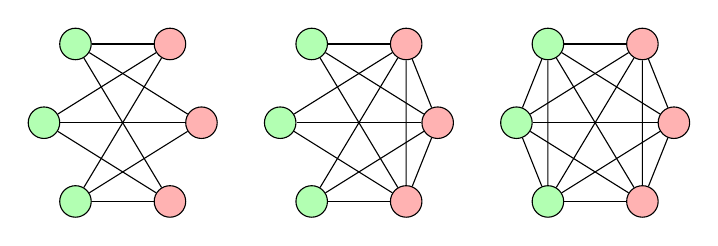
\begin{tikzpicture}[node distance=1.5cm, every node/.style={circle, draw,fill=red!30, minimum size=4mm}]
    % Bipartite communications
    \begin{scope}[local bounding box=graph1]
        % Left nodes
        \foreach \y in {0,2} {
            \node[fill=green!30] (L\y1) at (0.4,\y) {};
        }
        \node[fill=green!30] (L11) at (0,1) {};
        % Right nodes
        \foreach \y in {0,2} {
            \node (R\y1) at (1.6,\y) {};
        }
        \node (R11) at (2,1) {};
        % Edges between all left and right nodes
        \foreach \a in {0,1,2} {
            \foreach \b in {0,1,2} {
                \draw (L\a1) -- (R\b1);
            }
        }
    \end{scope}

    % One-sided communications
    \begin{scope}[shift={(3,0)}, local bounding box=graph2]
        % Left nodes
        \foreach \y in {0,2} {
            \node[fill=green!30] (L\y2) at (0.4,\y) {};
        }
        \node[fill=green!30] (L12) at (0,1) {};
        % Right nodes
        \foreach \y in {0,2} {
            \node (R\y2) at (1.6,\y) {};
        }
        \node (R12) at (2,1) {};
        % K_{3,3} edges
        \foreach \a in {0,1,2} {
            \foreach \b in {0,1,2} {
                \draw (L\a2) -- (R\b2);
            }
        }
        % Complete right subgraph
        \draw (R02) -- (R12) -- (R22) -- (R02);
    \end{scope}

    % Complete communications
    \begin{scope}[shift={(6,0)}, local bounding box=graph3]
        % Left nodes
        \foreach \y in {0,2} {
            \node[fill=green!30] (L\y3) at (0.4,\y) {};
        }
        \node[fill=green!30] (L13) at (0,1) {};
        % Right nodes
        \foreach \y in {0,2} {
            \node (R\y3) at (1.6,\y) {};
        }
        \node (R13) at (2,1) {};
        % K_{3,3} edges
        \foreach \a in {0,1,2} {
            \foreach \b in {0,1,2} {
                \draw (L\a3) -- (R\b3);
            }
        }
        % Complete left and right subgraphs
        \draw (L03) -- (L13) -- (L23) -- (L03);
        \draw (R03) -- (R13) -- (R23) -- (R03);
    \end{scope}
\end{tikzpicture}
\setlength{\belowcaptionskip}{-10pt}
\caption{The different kinds of communication networks we consider. From left to right: bipartite, one-sided and fully-connected networks. Note that even when communication is possible within $L$ or $R$, the matching is still between parties in $L$ (not within $L$ or $R$).} 
\label{fig:communication-networks}
\end{figure}


\noindent \emph{(Fully-connected network)} Parties are pairwise connected. This model is relevant in scenarios such as forming partnerships within a close-knit social group.

\noindent \emph{(One-sided network)} Parties are pairwise connected, except parties within $L$, which cannot communicate directly. This structure is applicable in contexts such as kidney donations, where privacy constraints prevent recipients from directly interacting with each other.

\noindent \emph{(Bipartite network)}
Only pairs of parties in $L \times R$ are connected.
This setup is relevant in cases such as matching international job applicants, where communication is restricted solely to potential matches across the two sets.

\vspace{0.1cm}


We remark that each model is strictly stronger than the previous one. 


The parties will then be running a protocol $\Pi$ where each party holds a preference list as input, and each party obtains as output its match (from the opposite side). In this setting, $\Pi$ achieves \emph{distributed stable matching} if the following properties hold:
\emph{(Termination)} Each party outputs a party on the opposite side to match with;
\emph{(Symmetry)} If party $u$ decides to match party $v$, then $v$ decides to match party $u$;
\emph{(Stability)} There are no blocking pairs.


\paragraph{Faults.}
%\paragraph{The modern society (Faults).} 
So far, we have defined the stable matching problem in a \emph{fault-free} setting. From now on, we assume a central adversary that may (permanently) corrupt up to $t_L$ parties in $L$ and up to $t_R$ parties in $R$. The corrupted parties become \emph{byzantine}: they may deviate arbitrarily (even maliciously) from the protocol. A party is \emph{honest} if it never became byzantine.
Our protocols will assume that the adversary is \emph{adaptive}: it may choose
to corrupt parties at any point of the protocol's execution. Our impossibility results, however, hold even against a \emph{static} adversary, which needs to choose which parties to corrupt at the beginning of the protocol's execution.


% \paragraph{Situationships and Polygamy (Refining the problem).} 
\paragraph{Refining the problem.} 
Byzantine parties require us to refine the definition of the stable matching problem. First, we need to take into account that our properties should only be concerned with the outputs of \emph{honest} parties. Second, the byzantine parties may choose not to participate in the protocol, preventing us from obtaining a maximal matching. Consequently, we adjust the previous properties as follows:

\vspace{0.1cm}
\noindent \emph{(Termination)} Every \emph{honest} party outputs: either a party on the opposite side \emph{or nobody}.

\noindent \emph{(Symmetry)} For two \emph{honest} parties $u$ and $v$, if $u$ decides to match $v$, then $v$ decides to match $u$.

\noindent \emph{(Stability)} There are no blocking pairs made of \emph{honest} parties.

\vspace{0.1cm}



%------------------------------------------
\begin{wrapfigure}{r}{3cm}
\centering
\includegraphics[width=3cm]{figures/not-enough-stable_cropped.pdf}
\vspace{-1.5cm}
\end{wrapfigure} 
%------------------------------------------



Note that these properties are not strong enough to lead to a \emph{relevant} matching: multiple honest parties may be matched to the same byzantine party (in the figure on the right, if the orange party is byzantine, the depicted matching satisfies 
symmetry and stability).
Therefore, we introduce an additional intuitive condition that prevents such scenarios:


\vspace{0.1cm}
\noindent \emph{(Non-competition)} If two honest parties output $u, v \in L \cup R$, then $u \neq v$.
\vspace{0.15cm}


We may now present the formal definition of byzantine stable matching. 
\begin{definition}[Byzantine Stable Matching ($\byzantineSM$)]
Consider a protocol $\Pi$ where every party in $L \cup R$ holds as input a preference list over the parties on the other side. Then, $\Pi$ achieves byzantine stable matching ($\byzantineSM$) if it satisfies the following even when up to $t_L$ parties in $L$ and $t_R$ parties in $R$ are byzantine: termination, symmetry, stability, non-competition.
\end{definition}


\paragraph{Cryptographic assumptions.}
%\paragraph{Screenshots (Cryptographic assumptions).}
As we will see, the solvability of $\byzantineSM$ in a given setting depends on whether we assume a trusted setup and cryptographic primitives. We will use the term \emph{unauthenticated setting} to refer to settings where no cryptographic assumptions are made. In contrast, we use the term \emph{authenticated setting} to refer to a setting where a public key infrastructure and a secure digital signature scheme are available. For simplicity of presentation, we assume that signatures are unforgeable. When replaced with real-world instantiations, our feasibility results in the authenticated setting still hold except for negligible probability (in the scheme's security parameter) against computationally-bounded adversaries.



\paragraph{Warm-up solution.} 
% \paragraph{Anti-Drama Dating App (A warm-up solution).} 
Synchronous networks come with communication primitives that often us to reduce $\byzantineSM$ to an offline problem. One such primitive is \emph{Byzantine Broadcast} ($\bb$) \cite{LSP82}.
\begin{definition}[Byzantine Broadcast ($\bb$)]\label{def:bc}
	Let $\Pi$ be a protocol where a designated party $\sender$ (the sender) holds a value $v_{\sender}$. 
    We say that $\Pi$ achieves Byzantine Broadcast ($\bb$) if the following hold even when up to some number $t$ of the parties are corrupted (alternatively for our setting, up to $t_L$ in $L$ and up to $t_R$ in $R$):
    (Termination) All honest parties output; 
    % and terminate;
    (Validity) If $\sender$ is honest, every honest party outputs $v = v_{\sender}$;
    (Agreement) Honest parties output the same value.
\end{definition}


A $\bb$ protocol allows the sender to disseminate its preferences so that all parties obtain identical views of them. If each party runs an invocation of $\bb$ to distribute its preferences, then by the end, all parties will have identical views of everyone's preferences. This enables them to run $\GaleShapley$ offline and obtain the same stable matching, thereby solving $\byzantineSM$. 
This provides us with the lemma below. We include the formal proof in Appendix~\ref{appendix:preliminaries}.

\begin{restatable}{lemma}{BroadcastEasy} \label{lemma:broadcast-easy}
Whenever $\bb$ is available, $\byzantineSM$ is solvable.
\end{restatable}

\section{Simplified Stable Matching}
For most of our impossibility results, we do not require the inputs to be complete preference lists: we rely only on parties' favorites. Therefore, we introduce the \emph{simplified stable matching} problem ($\simplifiedSM$), which mostly follows the same rules as $\byzantineSM$. The main difference is that a party's input is a party on the other side, not a preference list. If party $u$ has as input party $v$, we say that $u$'s \emph{favorite} is $v$. The stability property is then replaced by simplified stability:

\vspace{.1cm}
\noindent \emph{(Simplified stability)} If two honest parties are each other's favorites, they output each other.
\vspace{.1cm}

Our impossibility proofs will describe settings where a protocol cannot simultaneously achieve termination, symmetry, non-competition, and this simplified property. In Appendix \ref{appendix:simplified-stable-matching}, we show that $\simplifiedSM$ can be reduced to $\byzantineSM$, enabling us to state the following result.


\begin{restatable}{lemma}{SimplifiedReduction} \label{coro:to-simplified}
Whenever $\simplifiedSM$ is not solvable, $\byzantineSM$ is not solvable.
\end{restatable}

We finish with a helpful technical lemma
allowing our impossibility arguments to only focus on proving that $\simplifiedSM$ cannot be solved in settings with few parties. The lemma then generalizes our arguments to settings with more parties. The proof is enclosed in Appendix \ref{appendix:simplified-stable-matching}.
\begin{restatable}{lemma}{ReduceNumberLemma}\label{lemma:reduce-number}
Let $\Pi$ be a protocol solving $\simplifiedSM$, supporting up $t_L$ byzantine parties in $L$ and $t_R$ byzantine parties in $R$. Then, for any $0 < d \leq k = n/2$, there exists a protocol $\Pi'$ solving $\simplifiedSM$ on $2d$ parties ($d$ on each side) that supports up to $\lfloor \frac{t_L}{\lceil k / d \rceil} \rfloor$ byzantine parties on the left side and $\lfloor \frac{t_R}{\lceil k / d \rceil} \rfloor$ byzantine parties on the right side.
\end{restatable}

\section{Related Work}
% \alan{better to present the overview of the existing methodology related to our work before diving into details.
% e.g. There are many topics related to controllable 3D generation, including 3D representation, controllable generation and the design of editing scheme. }



% \subsection{Neural rendering and Gaussian Splatting}
% \subsection{基于3D gaussian的3D生成}
% \subsection{3D编辑}
\subsection{Neural Rendering and Gaussian Splatting}
% NeRF 凭借着它的高质量的视图合成能力成为了3D representation 中的热门研究话题. 
% 1. 讲radiance field很好,有很多工作提升
% 2.讲gaussian spaltting很好,做了什么改进,这种方法让什么成为可能
% radiance field 凭借在3D重建和视图合成中的强大的潜力成为3D representation 中的热门研究话题. NeRF作为一个里程碑式的工作,将高质量的视图合成成为可能。and its varients 致力于提升它的渲染质量, 训练和推理速度. Among them, 3D Gaussian Splatting(3DGS)采用point-based Radiance filed, 通过使用3D Gaussian primitives表示场景,通过 anisotropic splatting 和可谓渲染使高质量重建和realtime rendering 成为现实,with some varients致力于提升rendering quality, enhancing geometry,its ablity to 同时表示高质量的几何和纹理,让许多任务和应用有了解决方案,包括3D generation.
Radiance fields have become a popular research topic in 3D representation due to their powerful potential in 3D reconstruction and view synthesis. NeRF\cite{mildenhall2021nerf}, as a milestone work, made high-quality view synthesis possible. Its variants focus on improving rendering quality\cite{barron2021mip, barron2022mip,barron2023zip}, training and inference speed~\cite{muller2022instant,fridovich2022plenoxels,hedman2021snerg,SunSC22}, and generalization ability~\cite{wang2021ibrnet,yu2021pixelnerf,chen2021mvsnerf,johari2022geonerf}. Among them, 3D Gaussian Splatting (3DGS)~\cite{kerbl3Dgaussians} adopts a point-based radiance field, using 3D Gaussian primitives to represent scenes. Through anisotropic splatting and advanced rendering techniques, it enables high-quality reconstruction and real-time rendering. Some variants further enhance rendering quality and geometry~\cite{zhang2024rade,huang20242d, Yu2024GOF,lu2024scaffold,yu2024mip}, offering the ability to represent both high-quality geometry and textures, which provides solutions for various tasks and applications, including 3D generation.
% Novel view synthesis (NVS) has always been a hot topic in the field of computer vision. By using MLP to implicitly represent the scene, Neural Radiance Fields (NeRF) \cite{nerf} achieves realistic rendering. Subsequent works have imporved NeRF to enhance rendering quality \cite{barron2021mip, barron2022mip, wang2023f2}, reduce the number of training views \cite{yang2023freenerf,wang2023sparsenerf,niemeyer2022regnerf,wu2024reconfusion}, lessen dependence on camera poses \cite{lin2021barf,truong2023sparf,chen2023local,bian2023nope}, and improve both training and inference speeds \cite{muller2022instant,fridovich2022plenoxels,  hu2023tri, barron2023zip, hedman2021snerg, reiser2021kilonerf,reiser2023merf,SunSC22, chen2022tensorf}. 
% 为了解决上述问题,3DGS使用各向异性的高斯原语表示场景并引入光栅化进行渲染,提升了速度和渲染质量。一些方法聚焦于减少内存消耗、表面重建提高几何质量、将相机位姿与高斯场联合优化,以及使用扩散模型生成高斯场。
% 3D Gaussian Splatting (3DGS) \cite{kerbl3Dgaussians} employs anisotropic Gaussian primitives to represent scenes and introduces rasterization-based splatting rendering algorithm, enhancing both speed and rendering quality. Some methods focus on various aspects of improving Gaussian field representations, including rendering quality\cite{lu2024scaffold,yu2024mip, ren2024octree,li20243d,zhang2024pixelgs, yang2024spec}, enhancing geometric accuracy\cite{zhang2024rade,huang20242d, Yu2024GOF}, and increasing compression efficiency, \cite{chen2025hac,yang2024spectrally,lu2024scaffold,fan2023lightgaussian}, joint optimization of camera pose and gaussian fields \cite{fan2024instantsplat,Fu_2024_CVPR,schmidt2024noposegs}, as well 3D generation \cite{zou2024triplane, tang2023dreamgaussian,tang2024lgm,LaRa}. 


\subsection{2D Diffusion Priors Based 3D Generation}
\label{sec:related-2d-diffusion}
% 借助于text-to-image 的diffusion model的高质量的生成能力,一些 Multiview diffusion model可以被用来进行视图合成based on text/image and view condition. And 一些方法探索了基于广泛的2D diffusion prior进行3D generation. Some methods use SDS-loss based method to optimizae 3D representation from 2D diffusion prior, inwhich DreamGaussian use 3D Gaussian as representation and optimize in 2 minutes,这些方法时间消耗较大由于逐个场景的优化。Others methods use a feed-forward 方法来进行3D 生成 from 2D priors, LGM通过multiview diffusion model首先生成four views, then infer corresponding 3DGS from them. 这些方法都会受到multiview diffusion model多视图不一致的问题的限制,resulting in 3D不一致的几何和纹理。
% Leveraging the high-quality generation capabilities of text-to-image diffusion models\cite{rombach2022high}, some multi-view diffusion models facilitate view synthesis based on text/image and view conditions, enabling 3D generation using 2D diffusion priors. Some methods optimize 3D representations from these 2D priors using an SDS-loss-based approach or direct optimization from generated images. For instance, DreamGaussian optimizes 3D Gaussians with SDS-loss in just 2 minutes. However, these methods are computationally expensive due to scene-by-scene optimization. Alternatively, some methods adopt a feed-forward or denoising process for 3D generation from 2D priors. For instance, LGM generates four views through a multi-view diffusion model and subsequently infers the corresponding 3DGS. These 2D-prior-based methods are constrained by the inconsistencies of the multiview diffusion model, leading to misaligned 3D geometry and textures. and 由于multi-view images 生成的随机性,无法做到可控的生成.
Leveraging the high-quality generation capabilities of text-to-image diffusion models \cite{rombach2022high,saharia2022photorealistic,betker2023improving}, some multiview diffusion models \cite{liu2023zero,shi2023zero123++,shi2023mvdream,wang2023imagedream,li2023sweetdreamer,long2024wonder3d} enable view synthesis based on text/image and view conditions, facilitating 3D generation from 2D diffusion priors. Some methods optimize 3D representations from these 2D priors using an SDS-loss-based approach \cite{shi2023mvdream,liang2024luciddreamer,poole2022dreamfusion,wang2024prolificdreamer,tang2023dreamgaussian}or direct optimization~\cite{tang2025mvdiffusion++} from generated images. 
% For example, Dreamgaussian\cite{tang2023dreamgaussian} optimizes 3D Gaussians with SDS-loss in just 2 minutes.
However, these methods are computationally expensive due to scene-by-scene optimization. Alternatively, other methods adopt a feed-forward~\cite{xu2024grm, xu2024instantmesh,li2023instant3d,liu2024one,tang2025lgm,chen2025lara} or denoising process~\cite{wang2025crm,liu2024one++,xu2023dmv3d} for 3D generation from 2D priors. For instance, LGM generates four views through a multiview diffusion model and then infers the corresponding 3DGS. These 2D-prior-based methods are constrained by inconsistencies in the multiview diffusion model, leading to misaligned 3D geometry and textures, and due to the stochastic nature of multiview image generation, they lack controlled generation.
%先讲multiview diffusion,再讲把这些用于3D生成以及的问题
%diffusion很好,然后催生出来很好的text-2image, multiview diffusion model. 一些方法借助SDS的方法去做生成,dreamgs取得了不错的效果。 一些方法如LGM,通过feed forwad的方法得到3DGS,and lara 也同样支持从generative 的mv image得到3D,



\subsection{End-to-end 3D Generative Models}
\label{sec:related_3d}
% 一些方法构建large reconstruction model, 直接从单张图像中得到3D表示,而不需要依赖于2D diffusion先验。其中TripalneGaussian首先从单张图像中得到点云表示,再结合triplane融合纹理特征,得到最终的3DGS,    取得了SOTA的单图生3D效果。一些方法使用3D diffusion来实现3D生成。如3DShape2VecSet构建VAE将3D信息encode到latent set,then decode into mesh,and可采用diffusion model进行latent set的生成。一些方法同样探索了基于Gaussian Splatting的diffusion生成方式, 如GaussianCube通过构建规模的structured gaussian,通过3D U-Net based diffusion model to generate Gaussian from noise. These methods能更好的建模到3D data的分布,但不能做到以用户友好的方式进行可控生成和编辑。与之相比Our model同样适用diffusion model来学习3D信息的分布,但无需构造3DGS数据集,并且可以通过drag in 3D space 的方式来来进行可控生成。
Some methods \cite{tochilkin2024triposr,zou2024triplane,hong2023lrm} directly generate 3D representations from a single image without relying on 2D diffusion priors. For example, TriplaneGaussian~\cite{zou2024triplane} creates a point cloud from a single image, combines it with triplane fusion for texture, and produces the final 3DGS, achieving state-of-the-art single-image 3D results. Other approaches~\cite{zhang2024clay,zhang20233dshape2vecset,zhao2024michelangelo,gupta20233dgen,nichol2022point,muller2023diffrf} use 3D diffusion models, like 3DShape2VecSet~\cite{zhang20233dshape2vecset}, which encodes 3D information into a latent set and decodes it into a mesh, with diffusion models generating the latent set. Some approaches~\cite{zhang2024gaussiancube,zhou2024diffgs,he2025gvgen,xiang2024structured} also explore diffusion-based generation with Gaussian Splatting, such as GaussianCube~\cite{zhang2024gaussiancube}, which constructs structured Gaussian representations and uses a 3D U-Net-based diffusion model to generate Gaussians from noise. While these methods model 3D data distribution well, they lack user-friendly control for generation and editing. In contrast, our model leverages a diffusion model to learn 3D information distribution without needing a 3DGS dataset, offering controllable generation through 3D space manipulation.
%讲feed-forwad的生成,如TGS
%讲基于diffusion的,如3dshape2vec, clay, diffgs,gaussiancube, point-e

\subsection{Editing in 3D Generative Models}  
\label{sec: relatd_edit}
% (用prompt或者别的什么形式)edit in 2d space, 在投影到3D时会不一致
% interactive 3D, 需要两个模态之间的转换。需要2D diffusion先验。几何不一致,per-scene optimization
% MVdrag3D, 在3D空间编辑后还是要投影到2D空间
%我们的方法只需要完全在3D空间中,通过drag sparse seed points,得到不同的3DGS表示。
% 为了实现可控的3D生成和编辑,Sketch dream
% Sketch dream ,需要SDS。不是在3D空间中编辑,视角选择用户不友好。需要oprimization
% hyperdreamer, 只能改texture.
% APAP,edit on mesh, need sds
% interactive3D, need sds. 需要把3DGS转成NGP,per scene optimizaiton
% mvdrag3D 需要借助2D diffusion做编辑。需要SDS做refine.
% 为了实现可控的3D生成和编辑, Sketch-dream通过改变草图,使用SDS优化来实现想要的编辑,可以实现生动的编辑效果。However, 可控性is constrained due to 是在2D空间中编辑,在没有被选择的视角下不能得到用户想要的效果。 Interactive3D 直接在3D空间中对3DGS进行编辑,使用SDS优化,and convert the 3DGS representation into instantNGP. MVDrag 将3D空间中的drag操作投影到multiview image中,使用2D diffusion的编辑能力进行编辑,接着通过LGM得到编辑后的3DGS表示,then use SDS refine. 这些在3D空间中进行编辑能以用户友好的方式进行。 However,所有这些方法都需要借助2D generative先验,会导致几何不一致的问题as described in  Sec. 1, and need time-consuming optimization. 与之不同,我们的方法在3D空间中拉拽编辑稀疏的seed point clouds, 不需要2D generative先验,通过our seed-point-driven 策略得到编辑后的3DGS,而无需optimization.
To enable controllable 3D generation and editing, SketchDream~\cite{liu2024sketchdream} allows users to modify the sketch and achieve edits using SDS optimization for vivid results. However, its controllability is limited as user modifications are made in 2D space, which may not produce the desired effect for unselected viewpoints.  Interactive3D~\cite{dong2024interactive3d} directly edits 3DGS in 3D space using SDS optimization and predefined operations, converting the 3DGS representation into InstantNGP~\cite{muller2022instant} with further refine. MVDrag3D~\cite{chen2024mvdrag3d} projects 3D-space drag operations onto multiview images, using 2D diffusion editing capabilities, and infers the edited 3DGS through LGM~\cite{tang2025lgm}, followed by SDS refinement. These methods offer a more user-friendly experience. However, all of these methods rely on 2D generative priors, which may lead to geometric inconsistencies (as discussed in Sec. \ref{sec:related-2d-diffusion}), and require time-consuming optimization. In contrast, our method enables interactive manipulation of sparse seed points in 3D space, applying seed-point-driven deformation to modify the 3DGS without 2D priors or additional optimization, offering a more user-friendly editing experience.
% However, they all rely on 2D generative priors, leading to geometric inconsistencies as discussed in Sec. 1, and require time-consuming optimization. In contrast, our method edits sparse seed point clouds directly in 3D space,  achieving the desired 3DGS edits without the need for optimization.without relying on 2D generative priors,
%先讲一些2D的编辑方法,再讲3D编辑的方法。再说目前没有和我们一样的

%\newpage
\begin{figure*}[hbt]
  \centering
  \includegraphics[width=\textwidth]{figs/pipeline.pdf} 
  \caption{Overview of the framework.}
  \label{fig:overview}
\end{figure*}

\section{Method}
\subsection{Overview}
Our method, \textsc{Drangen3D}, takes an image as input and generate a 3D object represented by 3D Guassians with multi-view geometric consistency, allowing user interaction of editing the geometry during the process. As illustrated in Fig.~\ref{fig:overview}, we first train an Anchor-Gaussian (Anchor-GS) VAE that encodes complex 3D information into a latent space and decodes it into 3DGS, enabling subsequent generation in the latent space (Sec.~\ref{sec:anchor-vae}).  
%
Then, we propose Seed-Point-Driven Controllable Generation module for 3D generation from a single image. This module starts with the generation of the rough initial geometry represented by a set of sparse surface points, named seed points, where we can apply the editing by deforming the seed points. After that, a mapping module is designed to map the (edited) seed point information to the latent space, which can be decode to 3DGS subsequently (Sec.~\ref{sec:seed-point-driven}). 

% \todo{Note that we do not directly generate anchor points because: computational complex; easy to learn; generated anchor points contains noise that affect the final geoemtry}


% As illustrated in Fig.~\ref{fig:overview}, the framework of \textsc{Dragen3D} mainly consists of two parts. We first adopt an anchor-based approach to obtain 3D Gaussians and propose the Anchor-GS VAE that constructs 3D Gaussians by leveraging points sampled from 3D assets and rendered images.
% %
% Through the anchor-based representation, we can compress both geometric and texture information into a set of anchor latents, which is beneficial for latent generation, as described in Sec.~\ref{sec:anchor-vae}

% Then we generate a set of sparse seed points to control the anchor latents and thus deform the final output 3DGS, designing and utilizing the Seed-Anchor Mapping module, as described in Sec. \ref{sec:seed-point-driven}.

% Overall, combining anchor-based 3DGS VAE and seed-point-driven generation approach gives large flexibility in geometric control and deformation during the 3D generation process.

\subsection{Background}
\paragraph{Gaussian Splatting}
% 3D Gaussian Splatting represents 3D objects explicitly through radiance-based methods, leveraging high-degree shape and color features for multi-view synthesis. Its differentiable volume rendering properties make it suitable for image-to-3D object generation, allowing for the alignment of conditioned image textures. This generation process $G$ can be outlined as follows:
% \begin{equation}
%     G:\{C\}_{x',y'} \rightarrow {\{\mu,o,A,F\}}_p,
% \end{equation}
% where $\{C\}_{x',y'}$ is pixels of the input at $(w, h)$. 
% % \mc{need to use different symbols to describe pixal and gaussian positions}.
% $\mu$, $o$, $A$, and $F$ denote the position, opacity, covariance matrix, and spherical harmonic features of each Gaussian particle $p$, respectively. The discretized splatting rendering renders at $\{C\}_{x',y'}$:
% \begin{equation}
%     \displaystyle\sum_{i \in \mathcal{N}}  \alpha_i \boldsymbol{SH}(r|_{x',y'};F_i)                      \displaystyle\prod_{j=1}^{i-1} (1-\alpha_j )\rightarrow \{C\}_{x',y'},
% \end{equation}
% where $\alpha_i$ is the product of $o_i$ and the projected Gaussian density of where the kernel interacts with the ray in direction $r|_{x',y'}$ from the specific pixel at $(x',y')$, and $\boldsymbol{SH}$ denotes the color calculated with features $F_i$. 
% This is equivalent to computing a depth-and-opacity weighted average color of particles along the ray direction. Consequently, individual Gaussian points possess adequate geometric and chromatic information.
% \subsection{3DGS}
% gaussian splatting将静态场景表示为一组各向异性的3d gaussians,每个像素的颜色通过基于点的alpha混合渲染来获得,从而实现高保真度的实时新视角合成。
Gaussian splatting represents scenes as a collection of anisotropic 3D Gaussians. Each Gaussian primitive $\mathcal{G}_i$ is parameterized by a center $\mu \in \mathbb{R}^3$, opacity $\alpha \in \mathbb{R}$, color $c \in \mathbb{R}^{3(n+1)^2}$ which is represented by n-degree SH coefficients and 3D covariance matrix $\Sigma \in \mathbb{R}^{3 \times 3}$,which can be represented by scaling $s\in \mathbb{R}^3$ and rotation $r\in \mathbb{R}^4$.
% \begin{equation}
%   \mathcal{G}(x) = e^{-\frac{1}{2}(x-\mu)^T\Sigma^{-1}(x-\mu)}
%   \label{3dgs_define}
% \end{equation}

% 为了保持协方差矩阵的物理意义,它必须是半正定的。因此,将协方差矩阵分解为一个缩放矩阵S和一个旋转矩阵R,其中S和R分别使用一个缩放向量和一个四元数旋转向量来表示。
% To maintain the physical meaning of the covariance matrix, it must be positive semi-definite.Therefore, the covariance matrix $\Sigma$ can be decomposed into a scaling matrix $S$ and a rotation matrix $R$:
% \begin{equation}
%   \Sigma = RSS^T R^T
%   \label{3dgs_decomposed}
% \end{equation}

% 渲染时首先将3D gaussian投影到2D空间。给定视角变换W,可以计算得到2D协方差矩阵,其中J是the Jacobian of the affine approximation of the projective transformation.随后基于深度对覆盖一个像素的高斯进行排序,使用基于点的alpha混合渲染得到像素的颜色。
During rendering, the 3D Gaussian is first projected onto 2D space. Given a view transformation matrix $W$, the 2D covariance matrix $\Sigma'$ can be computed as :
$\Sigma' = JW\Sigma W^T J^T$, where $J$ is the Jacobian of the affine approximation of the projective transformation. Subsequently, the Gaussians covering a pixel are sorted based on depth. The color of the pixel is obtained using point-based alpha blending rendering:
\begin{equation}
  c = \sum_{i=1}^n c_i \alpha_i \prod_{j=1}^{i-1}(1-\alpha_i)
  \label{3dgs_render}
\end{equation}

\paragraph{Rectified Flow Model}
% Recitified flow modle有建立两个分布\pi_0, \pi_1之间mapping的能力,所以很适合我们的任务。给定x_0 ~ \pi_0 和 相对应的x_1 ~ \pi_1, 我们可以通过liner interpolation  得到 x(t) = (1-t) x_0 + t x_1 at timestamp t. And a vector filed v_sita parameterized by a neural network 被用来drive the flow from source distribution \pi_0 to target distribution \pi_1 by minimizing the conditional flow matching objective:
The Rectified Flow Model \cite{liu2022flow, lipman2022flow} has the capability to establish a mapping between two distributions, \( \pi_0 \) and \( \pi_1 \), making it well-suited for our task of mapping seed point latents to anchor latents. Given \( x_0 \sim \pi_0 \) and the corresponding \( x_1 \sim \pi_1 \), we can obtain \( x(t) = (1 - t) x_0 + t x_1 \) at timestamp \( t \in [0,1]\) through linear interpolation. A vector field \( v_{\theta} \) parameterized by a neural network is used to drive the flow from the source distribution \( \pi_0 \) to the target distribution \( \pi_1 \) by minimizing the conditional flow matching objective:
\begin{equation}
    L(\theta) = E_{t,x_0,x_1,y}||v_{\theta}(x_t, t,y) - (x_1 - x_0)||
    \label{eq:flow matching}
\end{equation}
Here, $v_{\theta}(x_t, t, y)$ is the predicted flow at time $t$ for a given point $x_t$, $y$ refers to the image  condition that guides the flow matching.
%\newpage
%%%%%%%%%%%%%%%%%%%%%%%%%%%%%%%%%%%%%%%%%%%%
\begin{table*}[t]
\centering
\begin{tabular}{@{}l|ccc|ccc|ccc@{}}
\toprule
\multicolumn{1}{c} {\textbf{Time} (\textit{s})}&
  \multicolumn{1}{l}{\textbf{4xA100}} &
  \multicolumn{1}{l}{\textbf{2xA100}} &
  \multicolumn{1}{l}{\textbf{A100}} &
  \multicolumn{1}{l}{\textbf{4xA6000}} &
  \multicolumn{1}{l}{\textbf{2xA6000}} &
  \multicolumn{1}{l}{\textbf{A6000}} &
  \multicolumn{1}{l}{\textbf{4xV100}} &
  \multicolumn{1}{l}{\textbf{2xV100}} &
  \multicolumn{1}{l}{\textbf{V100}} \\ \midrule
CPU Freezing (\textit{s}) & 21.49 & 10.32 & 4.96  & 15.23 & 9.11  & 3.35  & 29.41  & 14.50 & 6.90  \\
CPU Frozen (\textit{s}) & 33.58 & 16.15 & 7.79  & 43.69 & 29.48 & 11.24 & 74.96  & 38.56 & 19.23 \\
CPU Mem. dump (\textit{s}) & 31.30 & 15.02 & 7.28  & 42.1  & 28.59 & 10.88 & 70.30  & 36.17 & 18.10 \\
CPU Mem. write (\textit{s}) & 28.62 & 13.99 & 6.80  & 40.4  & 27.70 & 10.49 & 66.30  & 34.40 & 17.26 \\ \midrule
%
\sys Checkpoint (\textit{s}) & 55.09 & 26.49 & 12.78 & 58.93 & 38.61 & 14.60 & 104.40 & 53.08 & 26.18 \\
\sys Restore (\textit{s}) & 35.13 & 17.22 & 8.32  & 24.1  & 13.83 & 5.50  & 43.14  & 21.69 & 10.61 \\ \midrule
Checkpoint size (GB) & 41.01 & 20.46 & 9.94 & 39.98 & 19.97 & 9.75 & 40.03  & 19.97 & 9.81 \\ \bottomrule
\end{tabular}\par
\vspace{-0.5em}
\captionsetup{justification=centering}
\caption{Checkpoint and restore performance (in seconds) when scaling training of GPT-2 Small (124M) to multiple GPUs.\\Times are not comparable across GPU families.}
\label{tab:multi-gpu-checkpointing}
\end{table*}

%%%%%%%%%%%%%%%%%%%%%%%%%%%%%%%%%%%%%%%%%%%%%%%%
\begin{figure}[t]
    \centering
    \includegraphics[width=.9\columnwidth]{figures/H100_Lock_Checkpoint_vs_Restore_Unlock.pdf}
    \vspace{-.5em}
    \caption{In-memory GPU checkpoint/restore with H100. Similar results are observed with A100.}
    \label{fig:in-memory-checkpoint-restore}
\end{figure}
%%%%%%%%%%%%%%%%%%%%%%%%%%%%%%%%%%%%%%%%%%%%%%%%
\begin{figure*}[t]
  \centering
  \begin{subfigure}[b]{\columnwidth}
    \includegraphics[width=.9\textwidth]{figures/H100_Unified_Restore_Times.pdf}
    \label{fig:h100-unified-restore-times}
  \end{subfigure}
  \hfill
  \begin{subfigure}[b]{\columnwidth}
    \includegraphics[width=.9\textwidth]{figures/A100_Unified_Restore_Times.pdf}
    \label{fig:a100-unified-restore-times}
  \end{subfigure}
  \vspace{-1em}
  \caption{Time to restore for model training from a checkpoint with \sys for H100 and A100 GPUs.}
  \label{fig:unified-restore-times}
\end{figure*}
%%%%%%%%%%%%%%%%%%%%%%%%%%%%%%%%%%%%%%%%%%%%%%%%

\section{Evaluation} \label{sec:evaluation}%
%
Our evaluation seeks to answer the following questions:
\begin{itemize}[leftmargin=*,leftmargin=15pt,itemindent=0pt]
    \item How does \sys perform when checkpointing and restoring large language models? (\textsection{\ref{sec:eval:diff-models}})

    \item What are the scalability implications of using checkpointing and restoring with multiple GPU devices? (\textsection{\ref{sec:eval:scalability}})

    \item What are the dominant factors affecting the latency of checkpointing and restore operations? (\textsection{\ref{sec:eval:overhead}})

    \item Can \sys support checkpoint and restore with both CUDA and ROCm applications? (\textsection{\ref{sec:eval:rocm}})
\end{itemize}

\subsection{Experimental Methodology}%
%
\stitle{Evaluation Setup.}
We evaluate \sys on 10 servers with specifications described in \Cref{tab:server-configs}, running Ubuntu 22.04 with kernel version 6.2.0 (A100 and H100), 5.15.0 (V100 and A6000), and NVIDIA driver 565.57.01, CUDA 12.7, and CentOS Stream 9 with kernel 5.14 with ROCm 5.6 (MI210).

\stitle{Performance Measurements.} We measure the performance of checkpoint and restore operations using detailed statistics generated by CRIU~\cite{criu-statistics} about the time spent in different stages, and with external tools like \texttt{perf stat} to gather more detailed performance data. We run each experiment 10 times and calculate the mean and standard deviation of each value in the collected data. To analyze the overhead of checkpointing with \sys, we measure the following performance metrics for models of different sizes:

\begin{itemize}[leftmargin=*,leftmargin=10pt,itemindent=0pt]
    \item \textbf{Checkpoint time:} The total time to create a snapshot of the running GPU application.
    \item \textbf{Freezing time:} The time to suspend the application using \texttt{ptrace} seize and interrupt.
    \item \textbf{Frozen time:} The time during checkpointing when the application is not running.
    \item \textbf{Memory dump time:} The time to collect the CPU memory pages of running processes. This does not include the time to write this memory to storage.
    \item \textbf{Memory write time:} The time to save the memory state to persistent storage.
    \item \textbf{Restore time:} The time to restore both CPU and GPU state from storage, and to resume the application.
\end{itemize}

\stitle{Workloads and micro-benchmarks.} We evaluate the proposed checkpoint/restore mechanisms for multiple models of different sizes (listed below) and a set of ROCm micro-benchmarks~\cite{amd2024rocm} representing common HPC workloads for AMD GPU~(\textsection{\ref{sec:eval:rocm}}). For NVIDIA GPUs we use the following models:

\begin{itemize}[leftmargin=*,leftmargin=10pt,itemindent=0pt]
    \item \textbf{LLaMA} \textbf{3.2} (1B, 3B) and \textbf{3.1} (8B)

    \item \textbf{GPT-2} with 124M, 355M, 774M, 1.5B parameters

    \item \textbf{BERT} Base (110M) and Large (340M) models
\end{itemize}
%
\subsection{\sys Performance with Deep Learning Models}
\label{sec:eval:diff-models}
%
We evaluate the performance of GPU checkpoint and restore operations with multiple model training workloads of different sizes. The results in~\Cref{fig:in-memory-checkpoint-restore} show that the time required to checkpoint the GPU state into host memory increases significantly for models with large number of parameters.
For instance, checkpointing and locking operations for the GPT-2 Small model (124M parameters) take an average of 4.9 seconds and 240 ms, respectively. In comparison, for a larger model such as GPT-2 XL (1.5B parameters), these operations require an average of 28 seconds and 500 ms, respectively.
The time to restore the GPU state from host memory increases gradually, with 2.5 seconds for GPT-2 Small and 11 seconds for GPT-2 XL, while the unlock time remains consistent for both models at approximately 160 ms.
We observe similar results with both A100 and H100 GPUs, highlighting the crucial impact memory bandwidth has on the performance of GPU checkpointing operations.
Several techniques have been proposed to address this problem, such as data compression and on-demand parallelism~\cite{yang2024on-demand}. Incorporating such techniques could further improve the efficiency of checkpoint/restore operations, especially for large-scale models.

~\Cref{fig:unified-restore-times} shows the unified restore time (the time to restore the combined CPU-GPU state) for models with different sizes with both H100 and A100 GPUs. The time required to restore the GPU state makes up a significant portion of the total restore time for small models, but becomes a relatively lesser portion for larger models. These results demonstrate that the restore time is also affected by the available bandwidth for CPU-GPU memory transfers, as well as the speed at which checkpoint data is loaded from disk into host memory.
The performance results and checkpoint sizes shown in \Cref{tab:combined-checkpoint-restore-times} suggest that the differences in performance between the experiments with H100 and A100 GPUs can be attributed not only to advancements in GPU hardware architecture but also to the critical role of the available CPU resources.

%%%%%%%%%%%%%%%%%%%%%%%%%%%%%%%%%%%%%%%%%%%%%%%%
\begin{table}[t]
\centering
\renewcommand{\arraystretch}{.9} % Reduce row height for tighter spacing
\begin{tabular}{@{}c|rrr@{}}
\toprule
\textbf{Model} & \textbf{Total (GB)} & \textbf{GPU (\%)} & \textbf{CPU (\%)} \\ \midrule
BERT-B~~(110M)  & 5.22  & 82.38\%  & 17.62\% \\
GPT2-S~~(124M)  & 10.32 & 89.15\%  & 10.85\% \\
BERT-L~~(340M)  & 9.90  & 90.91\%  & 9.09\%   \\
GPT2-M~(355M)  & 19.57 & 91.31\% & 8.69\%   \\
GPT2-L~~(774M)  & 35.39 & 90.99\% & 9.01\%  \\
LLaMA 3.2~~~(1B) & 14.81 & 92.37\% & 7.63\%  \\
LLaMA 3.2~~~(3B) & 29.54 & 95.70\%  & 4.30\%   \\
LLaMA 3.1~~~(8B) & 55.89 & 97.35\% & 2.65\%  \\
GPT2-XL~(1.5B) & 60.12 & 96.02\% & 3.98\%  \\ \bottomrule
\end{tabular}
\vspace{-.5em}
\caption{The total unified checkpoint size (in GB) and the corresponding proportions of GPU memory and CPU state, respectively, for various models running on H100 GPU. We observe similar results with A100 GPU.}
\label{tab:cpu-to-gpu-state-comparison}
\vspace{-1.5em}
\end{table}
%%%%%%%%%%%%%%%%%%%%%%%%%%%%%%%%%%%%%%%%%%%%%%%%

\Cref{tab:cpu-to-gpu-state-comparison}  shows the total \sys checkpoint sizes for various models on both A100 and H100 GPUs, along with a breakdown of GPU memory and CPU state proportions. A key insight is the dominance of GPU memory in overall checkpoint size, consistently exceeding 80\% and often surpassing 90\% for larger models like LLaMA 3.1 (8B) and GPT2-XL (1.5B). These results further emphasize the importance of efficient CPU-GPU memory transfers in optimizing the performance of checkpointing and restore operations.

%%%%%%%%%%%%%%%%%%%%%%%%%%%%%%%%%%%%%%%%%%
\subsection{Multi-GPU Checkpointing Performance}
\label{sec:eval:scalability}
%
We evaluate the scalability of \sys by running an experiment designed to train a large language model (GPT-2) across 1x, 2x, and 4x GPUs of V100, A6000, and A100 types, using data parallelism to distribute the workload.
\Cref{tab:multi-gpu-checkpointing} shows that the checkpoint size increases with the number of GPUs, as each GPU stores its own copy of the model parameters.
For instance, the checkpoint size for 1, 2, and 4 A100 GPUs is $\approx10$, $\approx20$, and $\approx40$ GB, respectively.
This increase in checkpoint size reflects the increasing amount of intermediate model state that is saved as the number of GPUs increases.
The freezing, frozen, memory dump and memory write times also increase with the number of GPUs, likely because more time is spend on handling the larger checkpoint data with additional GPUs.
For example, as the number of A100 GPUs increases, creating a unified CPU-GPU snapshot requires scanning more memory pages.
A single GPU requires $\approx7$ million pages scanned, two GPUs require $\approx15$ million, and four GPUs require $\approx28$ million. Our experiments demonstrate that \sys efficiently scales as the number of GPUs and data-parallel replicas increase. We observe that checkpointing and restore times scale near linearly as we increase the number of GPUs from 1 to 4 across different GPU types.

\subsection{Checkpoint and Restore Latency}%
\label{sec:eval:overhead}%
We analyze the overhead of checkpoint and restore operations of \sys by measuring the latency during these processes for LLaMA 3.1 and GPT2-XL model training workloads on H100 and A100 GPUs. The results in ~\Cref{tab:combined-checkpoint-restore-times} highlight the performance differences between the H100 and A100 GPUs, as well as the impact of additional CPU and memory resources on reducing overhead during the checkpoint and restore operations with \sys. The primary factors affecting \sys's checkpoint and restore performance are:

\begin{itemize}
    \item \textbf{GPU count}: Increasing the number of GPUs leads to increased checkpoint size and latency;
    \item \textbf{CPU-GPU bandwidth}: The speed of data transfers between the CPU and GPUs directly affects checkpointing and restoring speed;
    \item \textbf{GPU memory usage}: Larger models with more parameters have higher checkpoint and restore latencies.
\end{itemize}

\begin{figure}[t]
  \centering
  \includegraphics[width=\columnwidth]{figures/MI210_Unified_Checkpointing_Times.pdf}
  \vspace{-2.5em}
  \caption{Breakdown of the \sys checkpointing time for HPC benchmarks running on AMD MI210 GPU.}
  \label{fig:amd-gpu-checkpointing}
  \vspace{-.5em}
\end{figure}
%%%%%%%%%%%%%%%%%%%%%%%%%%%%%%%%%%%%%%%%%
\begin{table}[t]
\centering
\begin{tabular}{lr}
\toprule
\textbf{Benchmark} & \textbf{Checkpoint Size}
\\ \midrule
Binomial Option Pricing       & 305~MB \\
Bitonic Sort                  & 614~MB \\
Discrete Cosine Transform     & 1.2~GB \\
1D Haar Wavelet Decomposition & 333~MB \\
Fast Walsh Transform          & 307~MB \\
Floyd Warshall                & 484~MB \\
Prefix Sum                    & 306~MB \\
Recursive Gaussian            & 311~MB \\
Histogram                     & 16.64 GB \\
Matrix Multiplication         & 19.88 GB \\
Convolution                   & 13.83 GB \\
\bottomrule
\end{tabular}
\caption{\sys checkpoint sizes of ROCm benchmarks.}
\label{tab:rocm-benchmark-checkpoints}
\vspace{-1em}
\end{table}

%%%%%%%%%%%%%%%%%%%%%%%%%%%%%%%%%%%%%%%%%
\subsection{\sys Support for ROCm Devices}
\label{sec:eval:rocm}

In addition to support for CUDA, to demonstrate the checkpointing functionality of \sys for AMD GPUs, we evaluate its performance using a set of ROCm HPC micro-benchmarks. These benchmarks provide a set of workloads representative of typical HPC applications, allowing us to analyse \sys's ability to effectively checkpoint and restore GPU state across different computational patterns. \Cref{fig:amd-gpu-checkpointing} shows the frozen, memory dump, and memory write times during checkpointing for each benchmark. While most of the evaluated benchmarks have relatively small checkpoint size, typically ranging from under 500~MB to 1.2~GB, a few have significantly larger checkpoint sizes (Histogram, Matrix Multiplication, and Convolution), shown in \Cref{tab:rocm-benchmark-checkpoints}. This increase in checkpoint size directly correlates with longer freezing and memory dump times, as \sys must checkpoint larger amount of data. An interesting observation is the contrasting distribution of checkpoint data between host memory and GPU memory across these benchmarks. While more than half of the checkpoint size for the Convolution benchmark is attributed to AMD GPU state, Histogram and Matrix Multiplication have the majority of their state residing in host memory.

\section{Conclusions}

We extensively evaluated SAE features for Gemma~2 in the out-of-distribution scenario using a variety of established and custom datasets. On the bright side, we find good SAE features for answerability across these domains. However, we show from various angles that the standard SAE feature search fails in finding these features and hence in terms of generalization.
We hypothesize that this is due to both sub-optimal training objectives and feature splitting with complex concepts \cite{bricken2023monosemanticity, chanin2024absorption}.
This shows the need for better technology for evaluating SAE features before SAEs are robustly applicable in practice.

%A key issue for SAE probing could be feature splitting, a phenomenon where SAEs of different sizes learn features in different granularities, often splitting more general features into multiple more specialized features \citep{bricken2023monosemanticity, chanin2024absorption}. If abstract concepts like answerability are split into many separate features, this can cause problems for feature-based practical applications.

%\newpage~\newpage~\newpage~\newpage
\section{Limitations} 

In this work, we compared the effectiveness and interplay of SFT and RL-based methods, under fixed data constraints. In particular, we chose offline methods like DPO and KTO as the baseline implementation of the RL method because it eliminates the need for reward modeling or iterative finetuning. This means that the process of development is limited to collecting an offline dataset and fientuning it - making it the most fair comparable to SFT in terms of implementation effort, compute costs and annotation efforts. Since this baseline RL method shows optimal performance over SFT, we hope that this motivates future work to study more complex RL-based methods and their interplay with SFT. In addition, we used GPT4o annotation for synthetic data generation, and also for evaluating Summarization and Helpfulness, which could include potential biases inherited from the model. 

In addition, we limited the size of the model to under 10 Billion parameters, to keep the finetuning cost low enough to ignore as compared to the data annotation costs. In addition, it would be extremely compute resource intensive to run thousands of finetuning runs with larger model sizes like 70B parameters. We hope that future work would study the scaling trends of RL-based methods against different model sizes, and also study the compute-data trade-off in-depth.

%In this paper we emphasize the importance of AI technologies that reflect linguistic diversity and are inclusive, particularly of minority populations such as Black Americans in the United States. Specifically, we explore if large language model-based generative AI technologies support the unique needs of Black Americans with respect to communications in AAE. In doing so,
We recruited Black American study participants to provide their opinions about the generation of AAE in AI technologies, such as AI assistants, and make judgments about how effectively these systems produce AAE. We do not believe our study participants were exposed to any meaningful risks through this process, and we ensured that their remuneration was fair and above average (two and a half times the U.S. federal minimum wage) for their time. Any minor risks that our participants might have been exposed to were delineated in our application to the Institutional Review Board of \emph{redacted}, which was approved with a status of ``Exempt'' on \emph{redacted}. All study participants provided informed consent for their participation. All data utilized by the large language models in this study was anonymized; specifically, we used publicly available transcriptions of interviews with Black Americans from the CORAAL corpus, which was anonymous when we retrieved it online. Finally, we utilized AI code-writing assistance to develop our code used to prepare our data sets.




% \section*{Acknowledgments}

% Bibliography entries for the entire Anthology, followed by custom entries
%\bibliography{anthology,custom}
% Custom bibliography entries only
\bibliography{main}

\appendix
\label{sec:appendix}
\appendix
\beginsupplement
\clearpage
\onecolumn
\section{Further Methodological Details} \label{sec:appendix-methodol}
\FloatBarrier
\begin{figure*}[ht]
\captionsetup{justification=raggedright, singlelinecheck=false, skip=2pt}
\centering
\begin{subfigure}[t]{0.3\linewidth}
   
    \subcaption{}
    \includegraphics[width=\linewidth]{sections/images/biden.jpg}
\end{subfigure}
\hspace{1cm}
\begin{subfigure}[t]{0.31\linewidth}

   \subcaption{}
   \includegraphics[width=\linewidth]{sections/images/rock.jpg}
\end{subfigure}
\caption{\mybold{AI-Generated Images from New York Times Quiz} \normalfont{\textbf{A}. NYT's explanation for evidence pointing to this image as AI-generated is: ``Though the resemblance to President Biden is striking, he would not be wearing military fatigues as a civilian.''~\cite{nytimes2024deepfake} \textbf{B}. NYT's explanation for evidence pointing to this image as AI-generated is ``One giveaway in this image is the badge, which includes garbled text.''~\cite{nytimes2024deepfake}}}
\label{fig:nytimes}
\Description{AI-generated image of Joe Biden in a conference room and an AI-generated image of the Rock in military uniform in a mall.}
\end{figure*}
\begin{figure*}[ht]
\centering
\captionsetup{justification=raggedright, singlelinecheck=false, skip=2pt}
\begin{subfigure}[t]{0.65\textwidth}
    \caption{}
    \vtop{\vskip0pt\hbox{\includegraphics[width=\linewidth]{sections/images/refiningpipeline.jpg}}}
\end{subfigure}
\hspace{0.01\textwidth} 
\begin{minipage}[t]{0.23\textwidth}
    \begin{subfigure}[t]{\textwidth}
        \caption{}
        \vtop{\vskip0pt\hbox{\includegraphics[width=\linewidth]{sections/images/facerefine.jpg}}}
    \end{subfigure}
    \vspace{0.5cm}
    \begin{subfigure}[t]{\textwidth}
        \caption{}\hfill\vtop{\vskip0pt\hbox{\includegraphics[width=0.8\linewidth]{sections/images/handrefine.jpg}}}
    \end{subfigure}
\end{minipage}
 \caption{\textbf{Image generation process in Stable Diffusion} A. \normalfont{Four stage image generation pipeline where the image is first generated in SD1.5. The output image is then encoded as latent and upscaled to be re-generated in SDXL with ControlNets applied for pose consistency. This is passed to the face refiner \cite{comfyuiimpactpack} which detects dominant and background faces in the image via YOLOv8 \cite{yolov8} and re-generates them using an SDXL pipeline. Finally, the resulting image is passed to the hand refiner \cite{comfyuiimpactpack} which detects hands in the image via YOLOv8  and predicts the hand pose used to guide the re-generation of the hands. \textbf{B}. Faces in the image before and after the face refining process \textbf{C}. Hand refining process. The left image shows the initial generation of the hand. The center image shows a predicted skeleton for the hand that is used for a ControlNet that guides the re-generation of the hand shown in the image on the right.}}
\label{fig:refiningpipe}
\Description{4 stage image generation pipeline}
\end{figure*}
\FloatBarrier
\twocolumn
According to a New York Times (NYT) quiz, qualities that typically signify AI generation include missing fingers, misaligned eyes, repeated elements, and garbled or nonsensical details~\cite{nytimes2024deepfake}.  Examples are shown in \ref{fig:nytimes}. The NYT quiz also discusses qualities that may cause a real image to look AI-generated, such as repeated cropping and compression that often happens over social media.

A screenshot of the pipeline, along with images before and after refinement, is shown in Figure~\ref{fig:refiningpipe}.
\FloatBarrier

\FloatBarrier
Figure~\ref{fig:pose-comprehensive} displays more examples of the four pose complexities and their average accuracies.
\onecolumn
\begin{figure}[H]
\centering
\resizebox{0.85\textwidth}{!}{
% This ensures the figure fits the page
\begin{minipage}{\textwidth}
% Portraits
\begin{subfigure}{0.22\linewidth}
    \includegraphics[width=\linewidth]{sections/images/ff_portrait3_014.jpeg}
    \caption{Acc: 25\%}
\end{subfigure}
\hfill
\begin{subfigure}{0.22\linewidth}
    \includegraphics[width=\linewidth]{sections/images/sd_portrait3_003.jpg}
    \caption{Acc: 37\%}
\end{subfigure}
\hfill
\begin{subfigure}{0.22\linewidth}
    \includegraphics[width=\linewidth]{sections/images/ff_portrait1_002.jpeg}
    \caption{Acc: 66\%}
\end{subfigure}
\hfill
\begin{subfigure}{0.22\linewidth}
    \includegraphics[width=\linewidth]{sections/images/sd_portrait3_075.jpg}
    \caption{Acc: 80\%}
\end{subfigure}

\vspace{0.3cm}

% Full Body
\begin{subfigure}{0.22\linewidth}
    \includegraphics[width=\linewidth]{sections/images/mj_fullbody3_028.jpg}
    \caption{Acc: 37\%}
\end{subfigure}
\hfill
\begin{subfigure}{0.22\linewidth}
    \includegraphics[width=\linewidth]{sections/images/mj_fullbody3_012.jpg}
    \caption{Acc: 57\%}
\end{subfigure}
\hfill
\begin{subfigure}{0.22\linewidth}
    \includegraphics[width=\linewidth]{sections/images/mj_fullbody3_022.jpg}
    \caption{Acc: 66\%}
\end{subfigure}
\hfill
\begin{subfigure}{0.22\linewidth}
    \includegraphics[width=\linewidth]{sections/images/mj_fullbody3_029.jpg}
    \caption{Acc: 83\%}
\end{subfigure}

\vspace{0.3cm}

% Posed Groups
\begin{subfigure}{0.22\linewidth}
    \includegraphics[width=\linewidth]{sections/images/mj_pg3_017.jpg}
    \caption{Acc: 37\%}
\end{subfigure}
\hfill
\begin{subfigure}{0.22\linewidth}
    \includegraphics[width=\linewidth]{sections/images/mj_pg2_012.jpg}
    \caption{Acc: 57\%}
\end{subfigure}
\hfill
\begin{subfigure}{0.22\linewidth}
    \includegraphics[width=\linewidth]{sections/images/mj_pg3_003.jpg}
    \caption{Acc: 66\%}
\end{subfigure}
\hfill
\begin{subfigure}{0.22\linewidth}
    \includegraphics[width=\linewidth]{sections/images/sd_pg3_013.jpg}
    \caption{Acc: 83\%}
\end{subfigure}

\vspace{0.3cm}

% Candid Groups
\begin{subfigure}{0.22\linewidth}
    \includegraphics[width=\linewidth]{sections/images/mj_ng3_016.jpg}
    \caption{Acc: 31\%}
\end{subfigure}
\hfill
\begin{subfigure}{0.22\linewidth}
    \includegraphics[width=\linewidth]{sections/images/mj_ng2_007.jpg}
    \caption{Acc: 66\%}
\end{subfigure}
\hfill
\begin{subfigure}{0.22\linewidth}
    \includegraphics[width=\linewidth]{sections/images/mj_ng4_003.jpg}
    \caption{Acc: 75\%}
\end{subfigure}
\hfill
\begin{subfigure}{0.22\linewidth}
    \includegraphics[width=\linewidth]{sections/images/mj_ng3_005.jpg}
    \caption{Acc: 87\%}
\end{subfigure}

\end{minipage}
}
\vspace{-2mm}
\caption{\textbf{More examples of the four pose complexities and their average accuracies.} \normalfont{The first row shows Portraits, the second row Full Body images, the third row Posed Groups, and the last row Candid Groups.}}
\label{fig:pose-comprehensive}
\Description{Examples of AI-generated images in different pose complexities: Portraits, Full Body, Posed Groups, and Candid Groups, with participant accuracy percentages.}
\end{figure}
\FloatBarrier
\twocolumn
\clearpage
\subsection{Robustness Check: Dataset Comparison}

To ensure the validity of our conclusions, we conducted a robustness check comparing the results from our full dataset against a subset excluding data collected before May 10th, 2024. This comparison addresses potential biases introduced by the initial experimental design, which did not implement stratified randomization as mentioned in Section \ref{exp-design}.

Table~\ref{tab:accuracy-comparison-dataset} presents the accuracy metrics for both the full dataset and the dataset excluding pre-May 10th data. The table includes overall accuracy, as well as specific accuracy for AI-generated and real images, along with their respective 95\% confidence intervals.

\begin{table}[H]
\centering
\caption{Comparison of accuracy: Full Dataset vs. Dataset excluding data before May 10th}
\label{tab:accuracy-comparison-dataset}
\resizebox{\linewidth}{!}{
\begin{tabular}{lcccccc}
\hline
Dataset & \multicolumn{2}{c}{Overall} & \multicolumn{2}{c}{AI-generated} & \multicolumn{2}{c}{Real} \\
 & Accuracy & 95\% CI & Accuracy & 95\% CI & Accuracy & 95\% CI \\
\hline
Full Dataset & 0.75 & [0.74, 0.76] & 0.76 & [0.74, 0.77] & 0.73 & [0.71, 0.75] \\
Dataset excluding data before May 10th & 0.75 & [0.74, 0.76] & 0.76 & [0.75, 0.77] & 0.7201 & [0.70, 0.74] \\
\hline
\end{tabular}}
\Description{A robustness check by comparing accuracy in full dataset vs. dataset excluding data before May 10th}
\end{table}

Figure~\ref{fig:accuracy-comparison-dstaset} visualizes the distribution of image accuracies for both datasets. This comparison allows for direct observation of any potential shifts in accuracy distributions between the full dataset and the subset, excluding early data.
 This robustness check supports the validity of using the full dataset in our main analysis.

\begin{figure}[H]
\centering
\includegraphics[width=\linewidth]{sections/images/dataset_accuracy_distribution_comparison.jpg}
\vspace{-10mm}
\caption{Comparison of accuracies between the full dataset and the dataset excluding data before 10th data.}
\label{fig:accuracy-comparison-dstaset}
\Description{Figure compares the distribution of accuracy of images from the full dataset vs. from the dataset excluding data before May 10th}
\end{figure}

\clearpage
\onecolumn
\section{Curated and Uncurated AI-generated Images}

\begin{figure*}[!htb]
\centering
\resizebox{1.0\textwidth}{!}{ % Scale figure to 95% of text width
\begin{minipage}{\textwidth} % Ensures correct alignment
\captionsetup{justification=raggedright, singlelinecheck=false, skip=2pt}

% Row A

\begin{subfigure}[t]{0.23\linewidth}  
\subcaption{}
\vtop{\vskip0pt\hbox{\includegraphics[width=\linewidth]{sections/images/ff_portrait3_001.jpeg}}}
\end{subfigure}
\hfill
\begin{subfigure}[t]{0.23\linewidth}  
\subcaption{}
\vtop{\vskip0pt\hbox{\includegraphics[width=\linewidth]{sections/images/american_faculty1.jpg}}}
\end{subfigure}
\hfill
\begin{subfigure}[t]{0.23\linewidth}  
\subcaption{}
\vtop{\vskip0pt\hbox{\includegraphics[width=\linewidth]{sections/images/american_faculty2.jpg}}}
\end{subfigure}
\hfill
\begin{subfigure}[t]{0.23\linewidth}  
\subcaption{}
\vtop{\vskip0pt\hbox{\includegraphics[width=\linewidth]{sections/images/american_faculty3.jpg}}}
\end{subfigure}

\vspace{8pt} % Reduced spacing between rows

% Row B
\begin{subfigure}[t]{0.23\linewidth}  
\subcaption{}
\vtop{\vskip0pt\hbox{\includegraphics[width=\linewidth]{sections/images/ff_pg4_001.jpeg}}}
\end{subfigure}
\hfill
\begin{subfigure}[t]{0.23\linewidth}  
\subcaption{}
\vtop{\vskip0pt\hbox{\includegraphics[width=\linewidth]{sections/images/astronaut1.jpg}}}
\end{subfigure}
\hfill
\begin{subfigure}[t]{0.23\linewidth}  
\subcaption{}
\vtop{\vskip0pt\hbox{\includegraphics[width=\linewidth]{sections/images/astronaut2.jpg}}}
\end{subfigure}
\hfill
\begin{subfigure}[t]{0.23\linewidth}  
\subcaption{}
\vtop{\vskip0pt\hbox{\includegraphics[width=\linewidth]{sections/images/astronaut3.jpg}}}
\end{subfigure}

\end{minipage}
}
\vspace{-2mm}
\caption{\mybold{Example images generated by consistently photorealistic and consistently detectable prompts.} \normalfont{
\textbf{A.} Curated image generated with a consistently photorealistic prompt: ``American woman faculty portrait, not a close-up, blond." 
\textbf{B-D} Reprompted images generated with the same consistently photorealistic prompts. 
\textbf{E.} Curated image generated with a consistently detectable prompt: ``Persian woman astronaut in astronaut clothes, family photo with husband and two toddlers, high resolution, realistic." 
\textbf{F-H} Reprompted images of the same consistently detectable prompts.}}
\label{fig:goodandbadprompt}
\Description{Two example images where A shows a portrait image of an American woman faculty with few visible artifacts and B shows a Persian woman and her child and husband in a space suit with noticeable artifacts in all of their faces.}
\end{figure*}

\clearpage
\onecolumn
\section{Future Work on Videos}
\begin{figure*}[ht]
\centering
\resizebox{1.0\textwidth}{!}{ 
\begin{minipage}{\textwidth} 
\captionsetup{justification=raggedright, singlelinecheck=false, skip=2pt}

% Row A
\begin{subfigure}[t]{0.33\linewidth}  
\subcaption{}
\vtop{\vskip0pt\hbox{\includegraphics[width=\linewidth]{sections/images/out_7.jpg}}}
\end{subfigure}
\hfill
\begin{subfigure}[t]{0.33\linewidth}  
\subcaption{}
\vtop{\vskip0pt\hbox{\includegraphics[width=\linewidth]{sections/images/out_9.jpg}}}
\end{subfigure}
\hfill
\begin{subfigure}[t]{0.33\linewidth}  
\subcaption{}
\vtop{\vskip0pt\hbox{\includegraphics[width=\linewidth]{sections/images/out_11.jpg}}}
\end{subfigure}

\vspace{10pt} % Spacing between rows

\begin{subfigure}[t]{0.33\linewidth}  
\subcaption{}
\vtop{\vskip0pt\hbox{\includegraphics[width=\linewidth]{sections/images/out_13.jpg}}}
\end{subfigure}
\hfill
\begin{subfigure}[t]{0.33\linewidth}  
\subcaption{}
\vtop{\vskip0pt\hbox{\includegraphics[width=\linewidth]{sections/images/out_15.jpg}}}
\end{subfigure}
\hfill
\begin{subfigure}[t]{0.33\linewidth}  
\subcaption{}
\vtop{\vskip0pt\hbox{\includegraphics[width=\linewidth]{sections/images/out_17.jpg}}}
\end{subfigure}

\vspace{10pt} % Spacing between rows

\begin{subfigure}[t]{0.33\linewidth}  
\subcaption{}
\vtop{\vskip0pt\hbox{\includegraphics[width=\linewidth]{sections/images/out_19.jpg}}}
\end{subfigure}
\hfill
\begin{subfigure}[t]{0.33\linewidth}  
\subcaption{}
\vtop{\vskip0pt\hbox{\includegraphics[width=\linewidth]{sections/images/out_21.jpg}}}
\end{subfigure}
\hfill
\begin{subfigure}[t]{0.33\linewidth}  
\subcaption{}
\vtop{\vskip0pt\hbox{\includegraphics[width=\linewidth]{sections/images/out_23.jpg}}}
\end{subfigure}

\vspace{10pt} % Spacing between rows

% Row C

\begin{subfigure}[t]{0.33\linewidth}  
\subcaption{}
\vtop{\vskip0pt\hbox{\includegraphics[width=\linewidth]{sections/images/out_25.jpg}}}
\end{subfigure}
\hfill
\begin{subfigure}[t]{0.33\linewidth}  
\subcaption{}
\vtop{\vskip0pt\hbox{\includegraphics[width=\linewidth]{sections/images/out_27.jpg}}}
\end{subfigure}
\hfill
\begin{subfigure}[t]{0.33\linewidth}  
\subcaption{}
\vtop{\vskip0pt\hbox{\includegraphics[width=\linewidth]{sections/images/out_29.jpg}}}
\end{subfigure}

\end{minipage}
}
\vspace{-2mm}
\caption{\mybold{Example frames from an AI-generated video with a temporal anatomical implausibility.} \normalfont{
9 frames from a video generated by OpenAI's Sora diffusion-transformer model where the subject's right leg morphs into the left leg somewhere between E and J. Each frame is separated by 1/10 of a second. This particular artifact fits into the anatomical implausibility category of the taxonomy, but it's different from any anatomical plausibility seen in diffusion model-generated images. In particular, this implausibility has a temporal element: the transition from A to L involves the subject's right leg becoming her left in a split second, which does not fit with what we know about human anatomy.}}
\label{fig:sora}
\Description{9 frames from a video generated by OpenAI's Sora diffusion-transformer model where the subject's right morphs into the left leg somewhere between E and J. Each frame is separated by 1/10 of a second. This particular artifact fits into the anatomical implausibility category of the taxonomy, but it's different than any anatomical plausibility in diffusion model-generated images. In particular, this implausibility has a temporal element: the transition from A to L involves the subject's right leg becoming her left in a split second, which does not fit with what we know about human anatomy.}
\end{figure*}

% This is an appendix.

\end{document}
